\documentclass[a4paper,12pt]{article}

% Packages
\usepackage[utf8]{inputenc} 
\usepackage{amsmath, amssymb} 
\usepackage{graphicx}
\usepackage[hidelinks]{hyperref}
\usepackage{natbib} % For managing citations
\bibliographystyle{apalike} % Or any other preferred style
\usepackage{geometry} 
\usepackage{booktabs}
\usepackage{tabularx}
\usepackage{adjustbox}
\usepackage{float}
\usepackage{subfigure}
\usepackage{longtable}
\usepackage{array}
\usepackage{indentfirst}
\usepackage{subcaption}

\title{Demographics of Unemployment: An inspection through COVID-19}

\author{
    Zeynep Bozoklu\thanks{\parbox[t]{0.75\textwidth}{Department of Economics, Bogazici University, Turkey. Email: \href{mailto:zeynep.bozoklu@std.bogazici.edu.tr}{zeynep.bozoklu@std.bogazici.edu.tr}}} 
    \and 
    Can Portakal\thanks{\parbox[t]{0.75\textwidth}{Department of Economics, Bogazici University, Turkey. Email: \href{mailto:can.portakal@std.bogazici.edu.tr}{can.portakal@std.bogazici.edu.tr}}}
}



\date{\today}

\begin{document}

\setlength{\parindent}{1.5em} % Adjust the size of the indentation

\maketitle


\begin{abstract}
    \noindent The COVID-19 pandemic has been one of the most important events in contemporaneous social life. It had devastating, and heterogeneous, effects on different societies in terms of political, social, and economic contexts. In this study, by utilizing the latest available Survey of Income and Living Conditions panel and cross-sectional data of TurkStat between 2018 and 2021 (SILC), weekly \textit{Government Stringency Index for COVID-19} and \textit{Cumulative COVID-19 Cases per million} datasets; changes in the demographic structure of the unemployed population within the period of COVID-19 is deconstructed. Through descriptive plots and clustering analysis, it is shown that pandemic-driven unemployment in different demographic groups in terms of their age, gender, education, and profession were heterogeneous. Younger individuals (under 25) experienced a decreasing trend in unemployment during the early stages of the pandemic, while older workers (55+) faced a steadily increasing trend, which is partly in line with the related literature while there has not been found any significance about “shecession”, which was broadly discussed in the literature. This work concludes by emphasizing the need for targeted and differentiated policy measures to mitigate the adverse effects on vulnerable groups, including older workers, blue-collar employees, and individuals with lower educational attainment.

\end{abstract}

\noindent\textbf{JEL Classification:} J21, J64, J10, E24 \\

\noindent\textbf{Keywords:} Unemployment; COVID-19 Pandemic; Demographic Analysis; Panel Data Analysis; Labor Market

\section{Introduction}
\subsection{Background}
    The COVID-19 pandemic, which began in Wuhan China at the end of 2019, has been one of the multi-faceted crises of our societies in recent years. It had severely affected social, humanitarian, and economic phenomena. The contagious nature of the disease had a serious impact on people to avoid getting together to transact, consume, and more importantly, to produce; which all led to a shrinking in total economic activity. This shrinkage of economic activities in countries with COVID-19 cases has led to a global economic recession. According to the estimates of the International Labour Organization \cite{ilo2021}, there has been a loss of 255 million full-time jobs in 2020, which is approximately four times greater than that of the 2009 global financial crisis. Moreover, the global economy contracted by about 3.4\% in 2020, marking the worst peacetime recession since the Great Depression.

    \indent As a developing country, Turkey has been seriously affected by the pandemic as well. 
    
    \begin{frame}
    \scriptsize 
    \begin{table}[H]
        \centering
        \begin{tabular}{|c|c|}
            \hline
            \textit{Date}   & \textit{Event} \\ \hline
            \textbf{March 11th}    &  \textbf{First case detected} \\ \hline
            March 16th    & Public places closed \\ \hline
            March 19th    & \$15 billion economic stimulus package \\ \hline
            March 21th    & Nationwide curfew \\ \hline
            March 30th    & Entrance to major cities banned \\ \hline
            \textbf{April 3th} & \textbf{Major Lockdown} \\ \hline
            April 28th   & Short-term work permits \\ \hline
            May 5th    & Reopening of automotive factories \\ \hline
            May 17th    & Cash assistance programs \\ \hline
            \textbf{June 1st}   & \textbf{Restrictions began easing} \\ \hline
            \textbf{November 20th} & \textbf{Reintroduction of restrictions} \\ \hline
            \textbf{March 2021} & \textbf{Temporary easing of restrictions} \\ \hline
            \textbf{April 29th 2021 }   & Full lockdown \\ \hline
            June 2021    & Gradual reopening \\ \hline
        \end{tabular}
        \caption{Timeline of COVID-19 Pandemic in Turkey}
        \label{tab:timeline}
    \end{table}
\end{frame}


    \indent As it can be seen from the timeline table of the COVID-19 pandemic in Turkey, the first positive-tested case was seen on March 11th, 2020 in Istanbul and the first death related to COVID-19 was declared on March 15th, 2020. As preventive measures against the contagion risk, schools and universities were closed on March 16, 2020, and public events were suspended. Turkey also imposed travel bans on 68 countries such as China, Germany, and France. Moreover, a curfew was imposed on individuals over the age of 65 and those under 20. Weekend and public holiday lockdowns were implemented in many cities, especially in the biggest three: Istanbul, Ankara, and Izmir. At the industrial level, some of the industrial giants of Turkey, such as \textit{Ford Otosan, Toyota} and \textit{Hyundai} announced that they would suspend production in their factories at Kocaeli, Gölcük and Sakarya.

    \indent On the public policy side, the Ministry of Treasury and Finance of Turkey implemented a large-scale economic stimulus package, equivalent to about 12\% of GDP, including credit guarantees, tax deferrals, and low-interest-rate policies, which are thought to have helped mitigate the expected economic downturn. In extension, as it was stressed in \cite{demiralp2020}, an aggressive easing policy based on sizable bond purchases and credit growth was implemented during the first half of the year. The related data from the Central Bank of the Republic of Turkey (CBRT) shows another explicit clue for the expansionary monetary policy. It can be seen that credit growth exceeded 50\% in real terms, marking one of the highest rates globally during the pandemic period.

    \indent Taking these information into consideration, it can be observed that although the economies of developed countries around the world had shrunk by an average of 4.5\%, the economies of emerging markets and developing countries faced a 2.1\% contraction on average. On the other hand, Turkey’s real GDP grew by 1.8\% in 2020, marking the second-highest growth rate among G20 countries, surpassed only by China. Additionally, the unemployment rate in Turkey stood at 13.2\% in 2020, highlighting significant labor market pressures despite government support programs. Therefore, the overall economic impact on Turkey seems to be mixed.
 


\subsection{Conceptual and Theoretical Framework}
\indent Despite the fact that Turkey differs from many other countries in terms of economic performance during the pandemic and provides us with the necessary motivation to take a closer look at its performance during COVID, this does not alone, justify the need to study the pandemic-driven unemployment in Turkey, which is the focus of the paper. 

\indent Conceptually, unemployment itself directly affects income, consumption, and overall economic stability. A study by \cite{piacentini2024} shows that the pandemic exacerbated existing inequalities; hitting low-wage workers, minorities, and women particularly harder. In addition, the same work shows that low-wage and minority workers experienced higher unemployment rates, and women faced increased caregiving burdens, potentially leading to long-term effects on their labor market attachment and wage growth. Another study by \cite{hershbein2020} emphasizes that understanding labor market impacts is essential for designing effective interventions, such as targeted support for vulnerable groups, retraining programs, and reforms to address systemic disparities. In essence, unemployment may be a suitable proxy showing how different demographic groups interact with the economic implications of COVID-19. 

\indent In line with the background information provided above, the objective and theoretical framework of this study is going to be to assess the demographic shifts in trends in unemployment under COVID-19, by using recent available cross-sectional and panel data of TurkStat, to provide a descriptive analysis by tracking specific individuals and households captured by SILC Panel Data of TurkStat between 2018-2021 and lastly, to understand why the pandemic in Turkey has been unequal in terms of its impact on different groups, which is a factor that is affecting many aspects in terms of policy making or social life. In this regard, in order to frame our analysis centered on COVID-19, TurkStat data was classified as "pre-COVID" in 2018 and 2019, and "post-COVID" in 2020 and 2021. Descriptive plots for each factor and compositional data analysis for their joint effects were constructed. Following these applications, the findings show that:
\begin{enumerate}
    \item The pandemic’s impact on unemployment varied across age and gender groups. While the unemployment rate for individuals under 25 showed a decreasing trend in the early stages of the pandemic, those above 55 experienced a stable yet increasing trend. Additionally, male unemployment rates remained consistently higher than female rates, although the gap slightly widened during strict lockdown periods.

    \item Higher education levels provided relative protection against unemployment. University graduates and high school graduates exhibited stable unemployment trends, while primary and middle school graduates, along with vocationally educated individuals, faced more distinct fluctuations. The illiterate group seemed to be less affected, probably due to their concentration in sectors that were less impacted by lockdowns.
    
    \item Blue-collar workers, particularly those with low skills, experienced significant unemployment fluctuations during lockdown periods, while white-collar workers exhibited more stable trends. White-collar workers, especially high-skilled ones, were less vulnerable to job losses during the pandemic.

    \item Both k-means and hierarchical clustering methods identified some of the distinct phases of unemployment dynamics, with clusters emerging at key points, such as the onset of the pandemic and the easing of restrictions. The clusters reflected varying unemployment trends across demographic groups, which may emphasize the heterogeneous effects of the crisis.

    \item The clustering çanalyses imply the need for differentiated policy measures. Groups such as older males with vocational education, blue-collar workers, and those employed in the private tertiary sector were disproportionately affected, indicating the necessity for targeted support and tailored policy interventions during and after economic crises.
    
\end{enumerate}

In conclusion, while it may be appealing to draw causal links and propose related policy recommendations, certain findings in this paper deviate from the existing literature, indicating the necessity for further research using new and more comprehensive datasets.





\section{Literature Review}
\indent Since the first news about the COVID-19 pandemic began to spread, many articles and works have been published using economic theory and econometric methods and models. This newly-emerging vast literature also involved possible effects on changing labor market conditions in many different regions, sectors, and countries including Turkey. There are many valuable contributions to this vast literature that reveal the heterogeneous impact of COVID-19 on various demographic groups of households and individuals. To illustrate further, the work of \textbf{\cite{aygun2021}} reports that Turkish women who have children and do not have a high school degree constitute the most vulnerable group against unemployment and income losses while on the other hand, the detrimental labor market effects of having children or being a woman are smaller among the university degree holders. Furthermore, the same study depicts that men’s unemployment rate increased from 12.4\% to 13.8\% between March and July 2020. They hypothesize about two different possibilities that might be in play: 
\begin{itemize}
    \item That the employment protection policies were effective in keeping the unemployment rate under control for men
    \item That some men exit the labor force.
\end{itemize} 

\indent Their work further suggests that Turkish women’s unemployment rate decreased in the first couple of months of the pandemic but returned to its pre-pandemic rate in July. In addition, they show that the probability of income loss was higher among singles, women, the informally employed, less educated, and individuals who live with children or the self-employed. Another paper by \textbf{\cite{aldan2021}} reveals that the least educated individuals were the ones who have been negatively affected by the pandemic, relative to more educated individuals, nearly in all countries that were hit hard by the pandemic in terms of total cases and death. On the other hand a work by \textbf{\cite{aum2021}}, which focuses on labor market dynamics in South Korea shows that employment losses due to the pandemic in South Korea did not cause an increase in the unemployment rate due to the fall in labor force participation. Among these valuable contributions, there has been a consensus in the literature that the COVID-19 pandemic had a disproportionate impact on women’s socioeconomic outcomes. In order to emphasize this peculiarity of the Covid-19 recession, the term \textbf{"shecession"} has been introduced in policy discussions and in related literature.

\indent \textbf{However;} the consensus regarding "shecession" may not be robust in the sense that, there is mixed empirical evidence about it. To illustrate it with the examples from the literature:
\begin{itemize}
    \item \textbf{\cite{cortes2020}} for the US and \textbf{\cite{farre2020}} for Spain find that women were hurt more in the labor market compared to men.
    \item In contrast, some others do not find any differential effect between men and women, such as \textbf{\cite{milovanska2021}} for the US and \textbf{\cite{petrongolo2020}} for the UK.

\end{itemize}

Additionally, work by \textbf{\cite{crossley2020}} depicts that young individuals are expected to be hurt more since workers with tenure contracts keep their jobs and new entrants into the labor market are severely affected by the decline in the hiring rate.

In the same context, \textbf{\cite{hoehnvvelasco2021}} found that youngest and oldest workers were more affected compared to middle-aged workers in Mexico, which is in line with the finding of \textbf{\cite{cortes2020}} for the US, which revealed that less educated were disproportionately affected by the pandemic.

\indent On the other hand, \textbf{\cite{montenovo2020}} found an \textit{inverse U-shaped pattern}, meaning that higher educated workers could continue their jobs remotely and least educated workers were concentrated in essential industries where lockdown measures were not implemented. In terms of age, \textbf{\cite{aldan2021}} found a similar U-shaped pattern to that of the US; the impact of the pandemic was hardest across young (aged 15-24) and old (55+).


\section{Data}
\label{sec:data}
\subsection{Data Sources}

The data utilized in this research originate from two primary sources:

The first source is the Turkish Statistical Institute (TurkStat)\footnote{The data cannot be disclosed due to confidentiality agreements.}, which provided the Survey of Income and Living Conditions (SILC) Panel Dataset (2018--2021) and Survey of Income and Living Conditions (SILC) Cross-Sectional Datasets (2018, 2019, 2020, 2021). The panel dataset offers longitudinal data that track individual and household characteristics over time, while the cross-sectional datasets provide annual snapshots of demographic and socioeconomic data for a broader population. These datasets enable both dynamic and static analyses of unemployment trends.

The second source is Our World in Data (OWID)\footnote{The data is available at \href{https://ourworldindata.org/explorers/covid?country=~TUR&Metric=Stringency+index&Interval=Daily&Relative+to+population=false}{Our World in Data Explorer}.}, which contributed contextual data on the COVID-19 pandemic. This includes the Government Stringency Index for COVID-19, which measures government response levels throughout the pandemic and increases in value as governments enact strict measures.

\subsection{Data Overview}

\indent Summary of the variables selected from the SILC Panel Dataset is provided in Table~\ref{tab:key-vars}.

\begin{table}[h!]
\centering
\begin{tabular}{|l|l|p{8cm}|}
\hline
\textbf{Category} & \textbf{Variable} & \textbf{Description} \\ \hline
Identifiers & HH\_ID & Household ID \\ 
 & PERS\_ID & Person ID \\ \hline
Demographics & FB010 & Year of the survey \\ 
 & FK090 & Gender \\ 
 & FK070 & Age \\ 
 & FB110 & Marital Status \\ 
 & FE030 & Highest Level of Education Attained \\ \hline
Labor Force & FI340A:FI340L & Monthly main activity status (January--December) \\ \hline
Other Key Variables & FI140 & Main sector of employment based on NACE Rev.2 \\ 
 & FI145 & Establishment type (public/private) \\ 
 & FI070--FI120 & Employment Status \\ 
 & FI080--FI130 & Occupation Code of Main (Last) Job (ISCO-08) \\ \hline
\end{tabular}
\caption{Summary of Key Variables from the SILC Panel Dataset}
\label{tab:key-vars}
\end{table}

Identifiers are crucial for linking and tracking individuals across the dataset, and the analysis was conducted at the individual level. Most of the information was recorded yearly, with the exception of the variables from \textit{FI340A} to \textit{FI340L}, which captured the main activity status at the end of each month. This posed a significant constraint on the analysis: if an individual was unemployed earlier in the year and later employed by the end of the year, the data related to their last job was deleted. Consequently, only the data corresponding to the individual's status at the end of the year was retained. 

\textit{Main job} is retained due to its more detailed information, including key variables such as \textit{FI140} and \textit{FI145}. Additionally, individuals who experienced unemployment during the year were more likely to reenter employment in similar roles and sectors where they had prior experience aligning with the findings of \cite{IZA-DP16696}, who investigated occupational targeting strategies of unemployed workers and highlighted the role of occupation-specific experience in shaping reemployment prospects.





\section{Methodology}

\subsection{Preliminary Analysis}

The dataset utilized in this research included 2-year, 3-year, and 4-year panel data. For consistency, only the 4-year panel data was retained. To focus on individuals consistently participating in the labor force, participants who left the labor force during the study period were excluded. These exclusions helped control for factors unrelated to unemployment, such as retirement or voluntary withdrawal from the workforce.

After filtering, the final dataset consisted of 62,880 individual observations per year, spanning the period 2018--2021. However, when calculating monthly unemployment shares across demographic groups, the data is aggregated into 48 group-level points. This aggregation reduced the robustness of statistical modeling, limiting the feasibility of conducting regression analysis for robust causal inference. Consequently, the analysis relied on descriptive plots and clustering methods to provide meaningful insights into unemployment trends across demographic groups. For the purpose of the analysis, the years 2018 and 2019 are classified as the pre-COVID period, while 2020 and 2021 are designated as the COVID period.

\begin{table}[H]
\centering
\begin{tabular}{|c|l|}
\hline
\textbf{Code} & \textbf{Description} \\ \hline
1 & Wage and salaried employee working full-time \\ \hline
2 & Wage and salaried employee working part-time \\ \hline
3 & Self-employed working full-time \\ \hline
4 & Self-employed working part-time \\ \hline
5 & Looked for a job/Unemployed \\ \hline
6 & Apprentices, trainees, or unpaid work experience \\ \hline
7 & Retired, in early retirement, or has given up business \\ \hline
8 & Disabled or unfit to work \\ \hline
9 & In compulsory military service \\ \hline
10 & Fulfilling domestic tasks and care responsibilities \\ \hline
11 & Other inactive person \\ \hline
\end{tabular}
\caption{Main Activity Status Codes in SILC Panel Dataset}
\label{tab:activity-status}
\end{table}

The share of unemployed individuals within the labor force is calculated to determine unemployment rates. The main activity status codes in the dataset were referred to (Table~\ref{tab:activity-status}). The unemployment rate is calculated as the share of individuals who were unemployed (i.e., those marked with activity code 5: "Looked for a job/Unemployed") among all individuals in the labor force (i.e., those marked from 1 to 5).  The time series is then decomposed (Appendix~\ref{appendix:decomposition}) using moving averages, with the trend component forming the basis for subsequent analyses.



To analyze demographic differences, unemployed individuals are grouped by gender, age, education level, sector of employment, establishment type, employment status,  and occupation category at the monthly level. Age brackets are classified into five groups: \textless 25, 25--34, 35--44, 45--54, and 55+. Furthermore, education levels are directly used as they were categorized in the dataset: \textit{Illiterate, literate with no schooling, primary, middle, high school, vocational} and \textit{university-plus}. The employment status mapping also followed the dataset’s classification: \textit{paid employment, wage earner, employer, self-employed} and \textit{unpaid family worker}. Occupation categories are grouped into broader categories as \textit{high-skill} and \textit{low-skill}, \textit{white-collar} and \textit{blue-collar} jobs based on Eurofound coding standards(Table~\ref{tab:occupation-mapping}).

\begin{table}[h!]
\centering
\begin{tabular}{|l|l|}
\hline
\textbf{FI130 Codes} & \textbf{Broad Occupation Category} \\ \hline
1, 2, 3 & white\_collar\_hs (high-skill white-collar jobs) \\ \hline
4, 5 & white\_collar\_ls (low-skill white-collar jobs) \\ \hline
6, 7 & blue\_collar\_hs (high-skill blue-collar jobs) \\ \hline
8, 9 & blue\_collar\_ls (low-skill blue-collar jobs) \\ \hline
\end{tabular}
\caption{Broad Occupation Mapping (Source: \href{https://www.eurofound.europa.eu/en/coding-and-classification-standards-0}{Eurofound Coding Standards})}
\label{tab:occupation-mapping}
\end{table}

Sectors of employment were categorized into three broad groups (Table~\ref{tab:sector-mapping}).

\begin{table}[H]
\centering
\begin{tabular}{|l|l|}
\hline
\textbf{FI140 Codes} & \textbf{Sector} \\ \hline
01, 02 & Primary \\ 
03, 04, 05 & Secondary \\ 
06–18 & Tertiary \\ \hline
\end{tabular}
\caption{Three-Sector Model Mapping}
\label{tab:sector-mapping}
\end{table}

Descriptive plots are generated from the filtered panel dataset and the cross-sectional data. These plots, presented in Appendix~\ref{appendix:descriptive-plots}, offered an overview of trends across individual variables among the NUTS2-classified regions in Turkey. However, no analyses of interplays or interactions between these variables were conducted at this stage.

\subsection{Compositional Data Analysis}

To account for the joint effects of the variables, compositional data analysis is employed. As highlighted by \cite{jackson2015}, proportions reside in a constrained simplex space where components are non-negative and sum to one, limiting the effectiveness of conventional statistical tools. To address this, Centered Log-Ratio (CLR) transformation (Appendix~\ref{appendix:clr_math}), which maps compositional data into an unconstrained Euclidean space by expressing each component relative to the geometric mean, is applied. This transformation enabled a more robust exploration of patterns and relationships across variables and laid the foundation for clustering analysis. Additionally, transformed variables of centered log-transformation were plotted together with the Stringency Index, which is going to be discussed further in the \textit{Findings} section of the paper.

Following the application of the CLR transformation, clustering methods are employed to uncover patterns and groupings across the transformed data. Clustering allows for the simultaneous consideration of all compositional variables, capturing interrelationships that might be missed when analyzing variables independently. Specifically, two clustering approaches were explored in this paper: hierarchical clustering and k-means clustering. Then, clusters over time for each method were plotted for 2, 3, and 4 clusters (Appendix~\ref{appendix:clustering_methodology}). 



\subsection{Robustness Check}

To validate the stability of the clustering results, a bootstrap analysis is conducted. This involved resampling the dataset multiple times and reapplying the clustering methods to assess the consistency of the cluster assignments. Stability scores were computed for each cluster configuration, providing insights into the robustness of the identified clusters.

For both hierarchical clustering and k-means clustering, the following steps were performed:
\begin{enumerate}
    \item Generate $B$ bootstrap samples from the original dataset.
    \item Apply the clustering method to each bootstrap sample for $k = 2, 3, 4$ clusters.
    \item Calculate the stability score for each cluster by comparing cluster assignments across the bootstrap samples.
\end{enumerate}

The results of the bootstrap analysis are summarized in Figure~\ref{fig:robustness_check}, which shows the stability scores for different configurations. Higher scores indicate more stable and reliable clusters.

The robustness check ensured that the clustering results were not overly sensitive to variations in the dataset and provided confidence in the reliability of the clusters used for further analysis.

\begin{figure} [H]
    \centering
    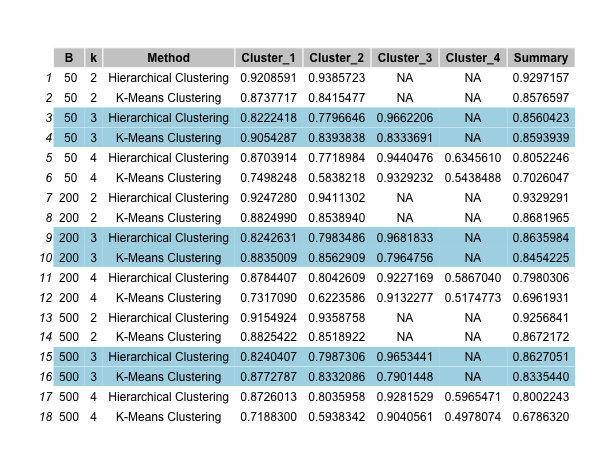
\includegraphics[width=1\linewidth]{highlighted_k3_with_cluster4_table.png}
    \caption{Cluster Stability Analysis via Bootstrapping}
    \label{fig:robustness_check}
\end{figure}




\section{Findings}
In this section, the main findings of the paper are presented. First, plots for trend-adjusted total unemployment in terms of gender, age groups, education levels, sectors, employment types, and worker profiles are obtained. Later, compositional data analysis and clustering methods are employed to observe how the available unemployment characteristics shifted roughly among different groups in the pre-COVID and post-COVID years. In addition, five major events or policy implementations which were thought to have affected the labor market dynamics, were depicted in the figures to better make eyeball estimations for potential overlaps in changes. The related events have been given in bold in (Table~\ref{tab:timeline}). There were no visible changes to identify in trends for separate variables in initial trend-adjusted plots. CLR-transformed versions with Stringency Index provided better insights and were retained in this section while trend-adjusted plots with no CLR transformation were placed in the Appendix~\ref{appendix:descriptive-plots}.


\begin{figure}[H]
    \centering
        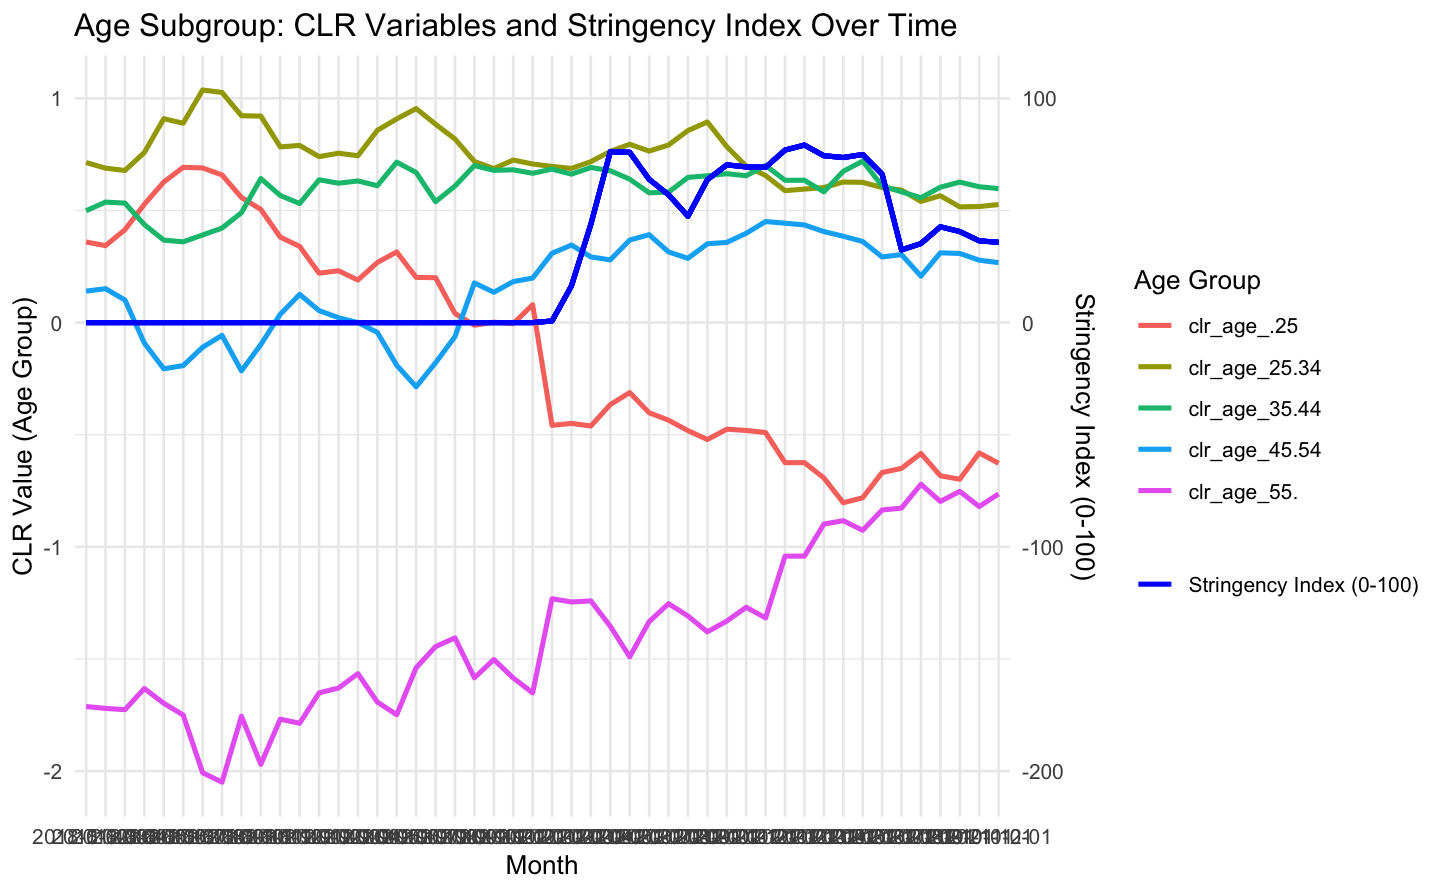
\includegraphics[width=1\linewidth]{clr_str_age.png}
        \caption{CLR-Transformed Age Groups and Stringency Index}
        \label{fig:clr_str_age}
\end{figure}

  As it can be seen in  (Figure~\ref{fig:clr_str_age}), the Stringency Index and CLR Transformed Trends for Unemployment of age groups plotted together and it can be seen that there are differing outcomes for differing groups with the change of enacted measures. In earlier times of the pandemic and until the end of its first year, unemployment had a decreasing trend for the population aged below 25 while there exists a more or less stable upward trend for the population above 55, slightly becoming steeper following the first year of the pandemic. Age groups between 25–54 followed trends that did not seem to overlap with any changes in the measures, suggesting that middle-aged individuals faced less pronounced changes in unemployment compared to younger and older cohorts. The Stringency Index, which was introduced in (Data~\ref{sec:data}), is presented in the figure since it properly illustrates the overall strictness of government lock-downs and measures, and here it shows sharp increases corresponding to the periods of stricter lock-downs and restrictions. The changes in trends for both the under-25 and 55+ age groups seem to be aligned with periods of heightened restrictions. From these results, it cannot be seen that the pandemic had a U-shaped impact on unemployment across age groups, with the youngest being less affected and the oldest workers being more affected, which is not exactly consistent with findings in the literature. This might be because of the fact that elder people tend to be less skilled and educated and younger people got out of the labor force and became inactive, waiting for the pandemic to come to an end, which has been commonly hypothesized in the related literature. \cite{aygun2021} . Additionally, in the case of Turkey, a significant increase in the employment of young labor force as motorcycle couriers might be the case. 


\begin{figure}[H]
    \centering
        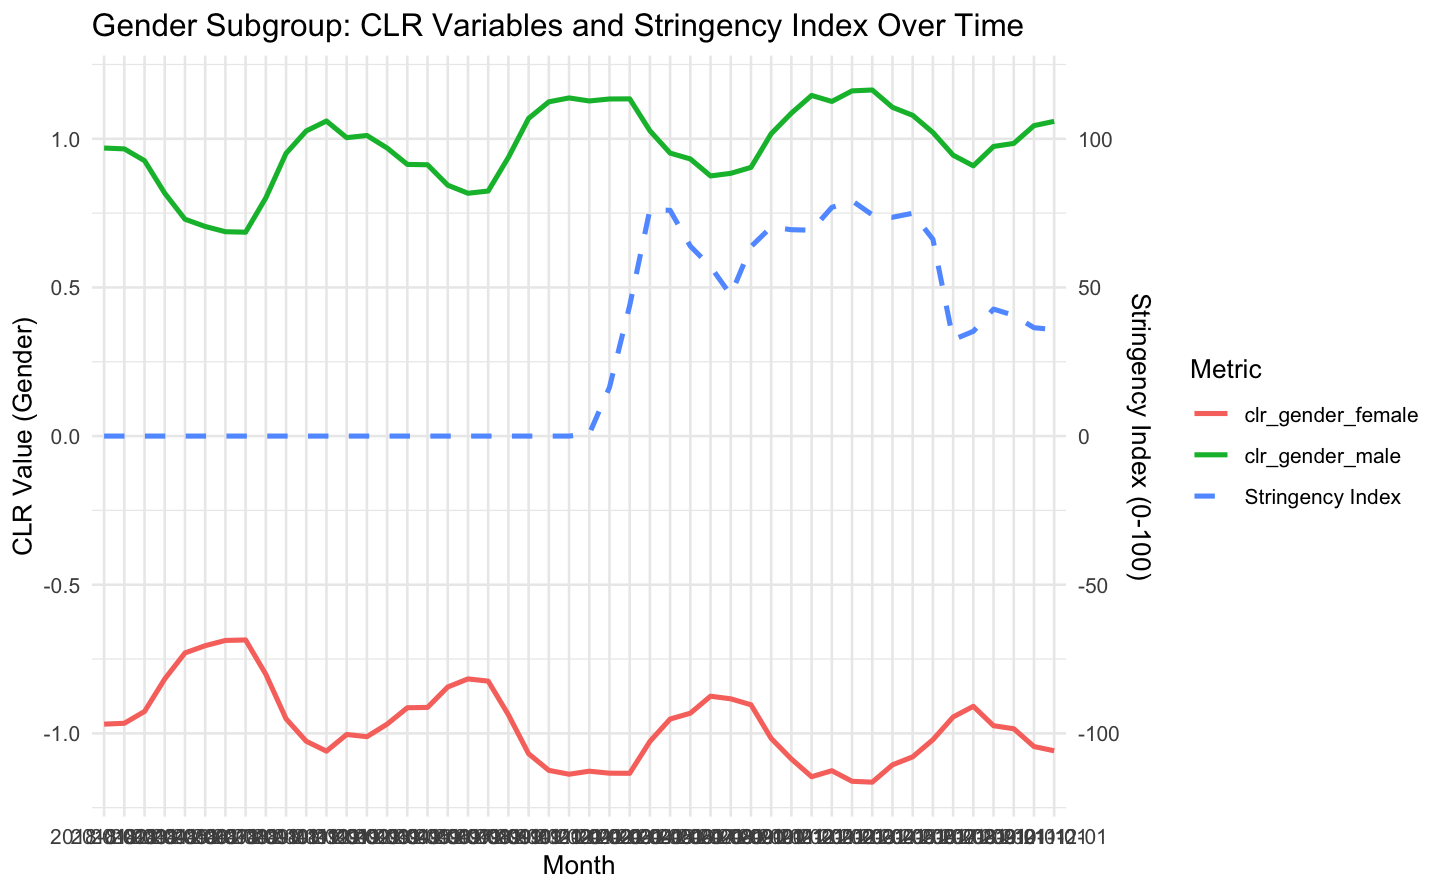
\includegraphics[width=\linewidth]{clr_str_gender.png}
        \caption{CLR-Transformed Gender and Stringency Index}
        \label{fig:clr_str_gender}
\end{figure}
In (Figure~\ref{fig:clr_str_gender}), the CLR values for males remain higher than those for females throughout the observed period, indicating that male unemployment rates were higher relative to females. The CLR values for females show a slight decline during key periods of lockdown, which may reflect a decrease in female unemployment relative to males. The Stringency Index slightly correlates with fluctuations in CLR values, particularly during periods of strict lockdowns, when the gap between male and female unemployment widened. Post-lockdown periods show some recovery in CLR values for females, but the gap between genders remains visible throughout the timeline.

    \begin{figure} [H]
        \centering
        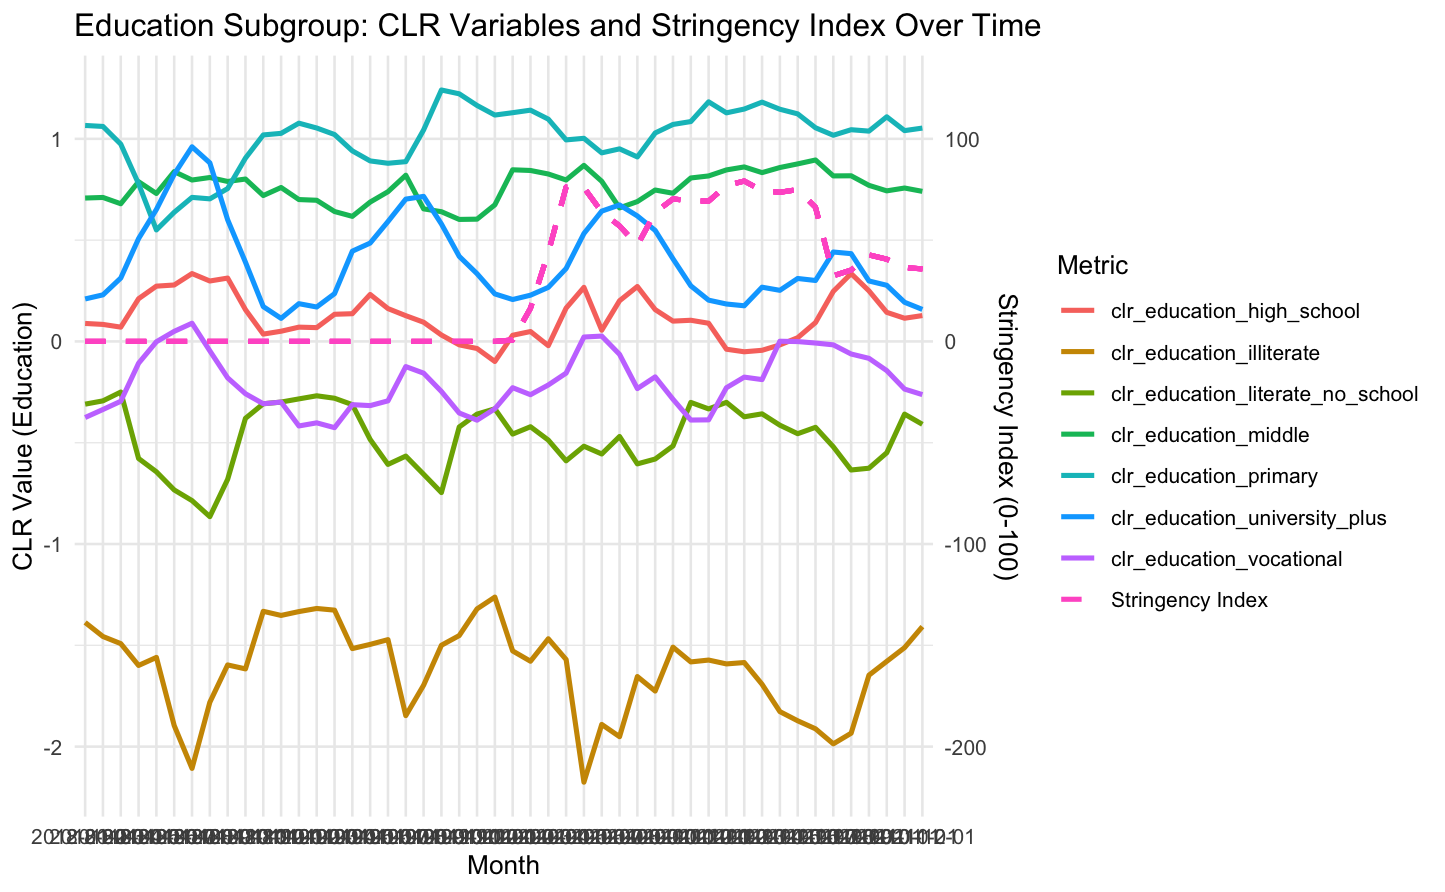
\includegraphics[width=1\linewidth]{clr_str_educ.png}
        \caption{CLR-Transformed Education Groups and Stringency Index}
        \label{fig:clr_str_educ}
    \end{figure}

The same analysis was conducted using education groups and worker profiles. The Stringency Index is, again, used to observe a correlation between government measures and their possible effects on unemployment of different groups. As it can be seen in (Figure~\ref{fig:clr_str_educ}), CLR values for 
University-plus and high school graduates exhibit relatively stable variability in time, indicating less impact on their unemployment rates. Primary and middle school graduates, as well as those with vocational education, show slight declines in CLR values during the pandemic, which may reflect decreasing unemployment rates.
The illiterate group has the lowest CLR values, which may indicate that they work in sectors that were not affected by lockdown measures.

    \begin{figure} [H]
        \centering
        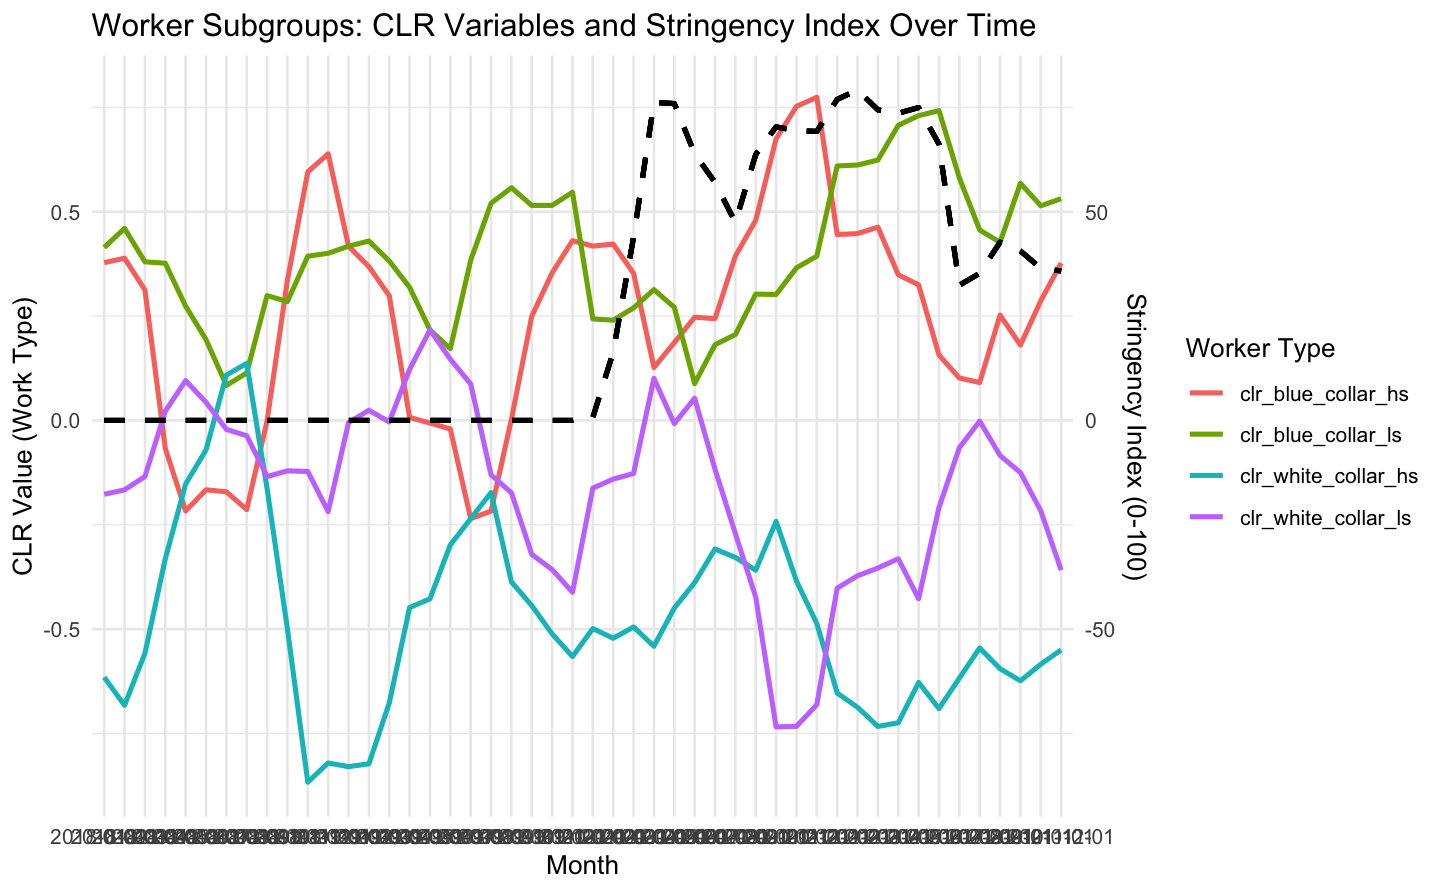
\includegraphics[width=1\linewidth]
        {clr_str_wp.png}
        \caption{CLR-Transformed Worker Profiles and Stringency Index}
        \label{fig:clr_str_wp}
    \end{figure}

On the other hand, the Stringency Index correlates with the increase in CLR values at the beginning of the pandemic, which may imply that lockdown measures increased unemployment in nearly all groups. For (Figure~\ref{fig:clr_str_wp}), the CLR values of white-collar workers in general, exhibit less fluctuations in CLR values during the pandemic period, compared to others.
The Stringency Index shows peaks during strict lockdown periods, which correspond to notable drops in CLR values for blue-collar workers. 




Following the CLR analysis on various demographic groups, time series plots were generated for 2, 3, and 4 clusters using both k-means and hierarchical clustering methods.


\begin{figure}[H]
    \centering
    \begin{minipage}{0.48\textwidth}
        \centering
        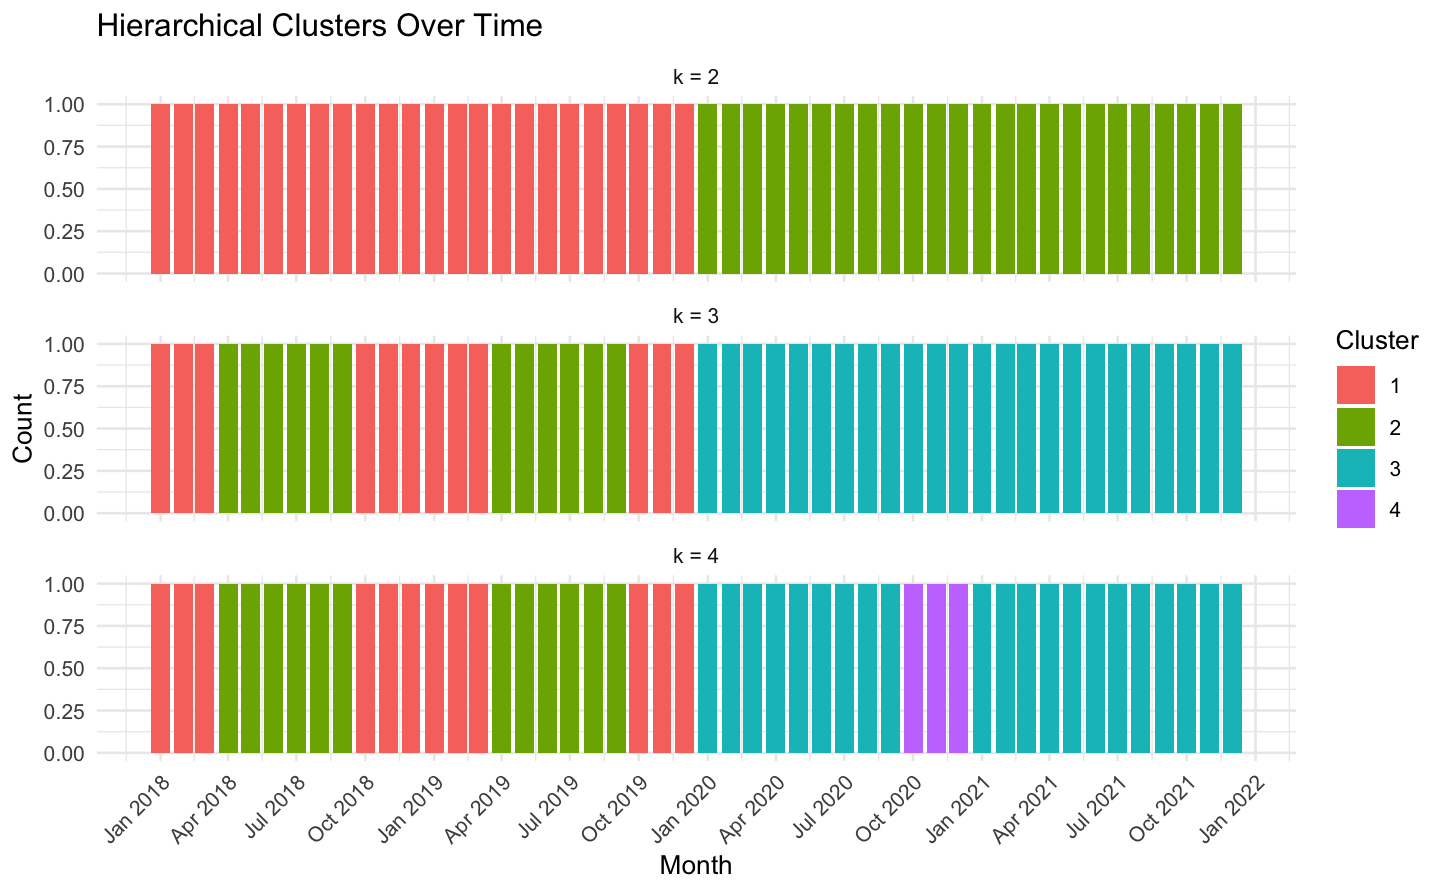
\includegraphics[width=\linewidth]{clr_hierclus.png}
        \caption{Different Clusters of Hierarchical Clustering Method}
        \label{fig:clr_hierclus}
    \end{minipage}
    \hfill
    \begin{minipage}{0.48\textwidth}
        \centering
        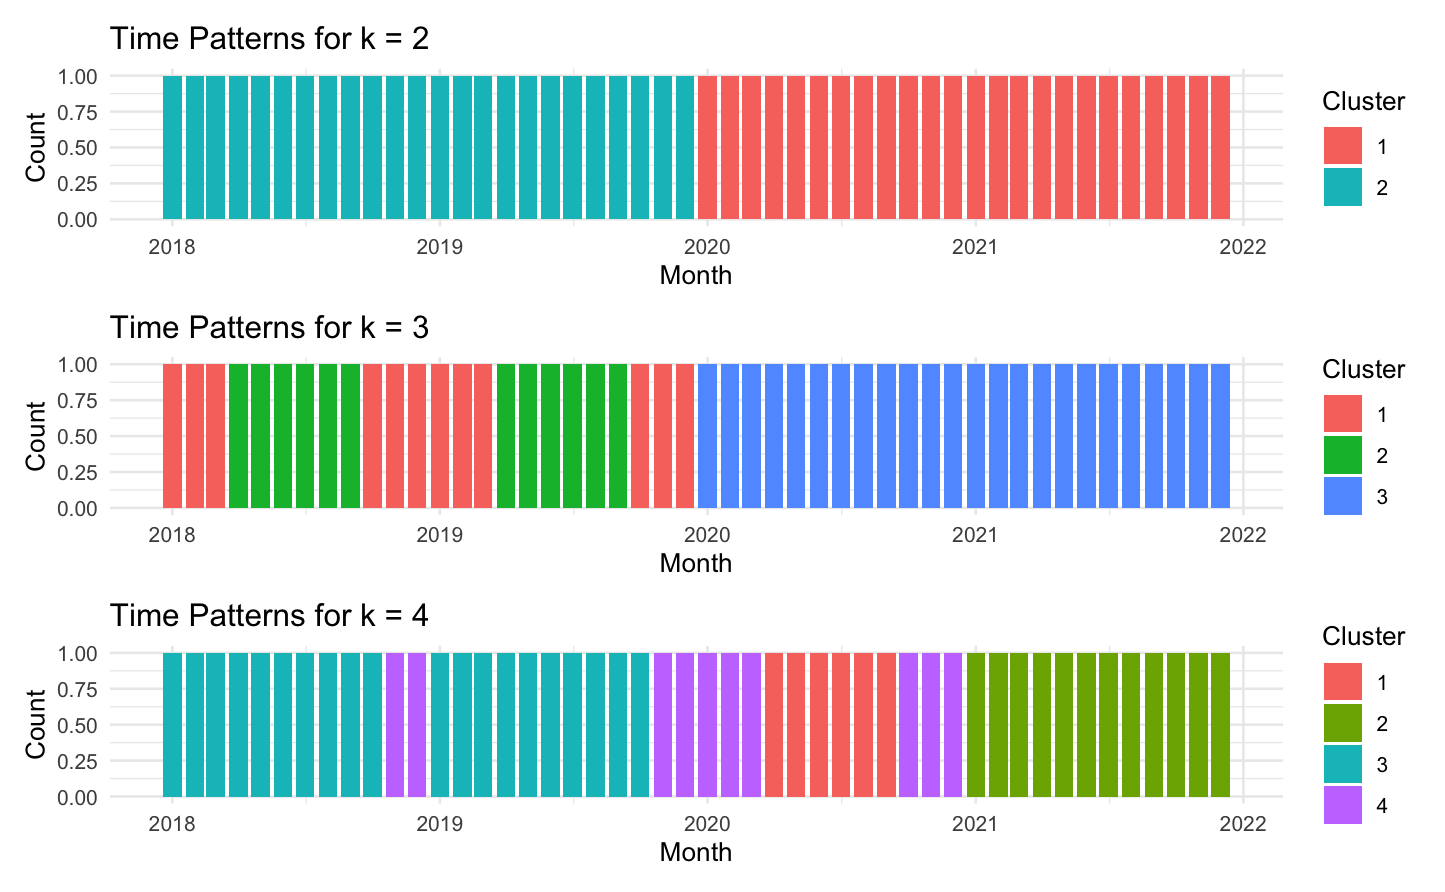
\includegraphics[width=\linewidth]{clr_kmean_123.png}
        \caption{Different Clusters of k-means for seed: 123}
        \label{fig:clr_kmean_123}
    \end{minipage}
\end{figure}


As it can be seen from both figures, (Figure~\ref{fig:clr_hierclus}, ~\ref{fig:clr_kmean_123}) for k = 2, the data is divided into two broad clusters, likely distinguishing between two primary time patterns of unemployment before and during the pandemic. For k = 3, three clusters emerge, offering a more detailed segmentation. The onset of the pandemic in early 2020 corresponds to the emergence of a new cluster, indicating a distinct change in labor market dynamics. For k = 4, the clustering becomes even more granular, identifying an additional pattern at the end of 2020, when economic recovery and easing restrictions began.

The transitions between clusters at key points in time may suggest that the method is useful for capturing changes in unemployment dynamics over different phases of the pandemic.

\begin{figure}[H]
    \centering
    \begin{minipage}{0.48\textwidth}
        \centering
        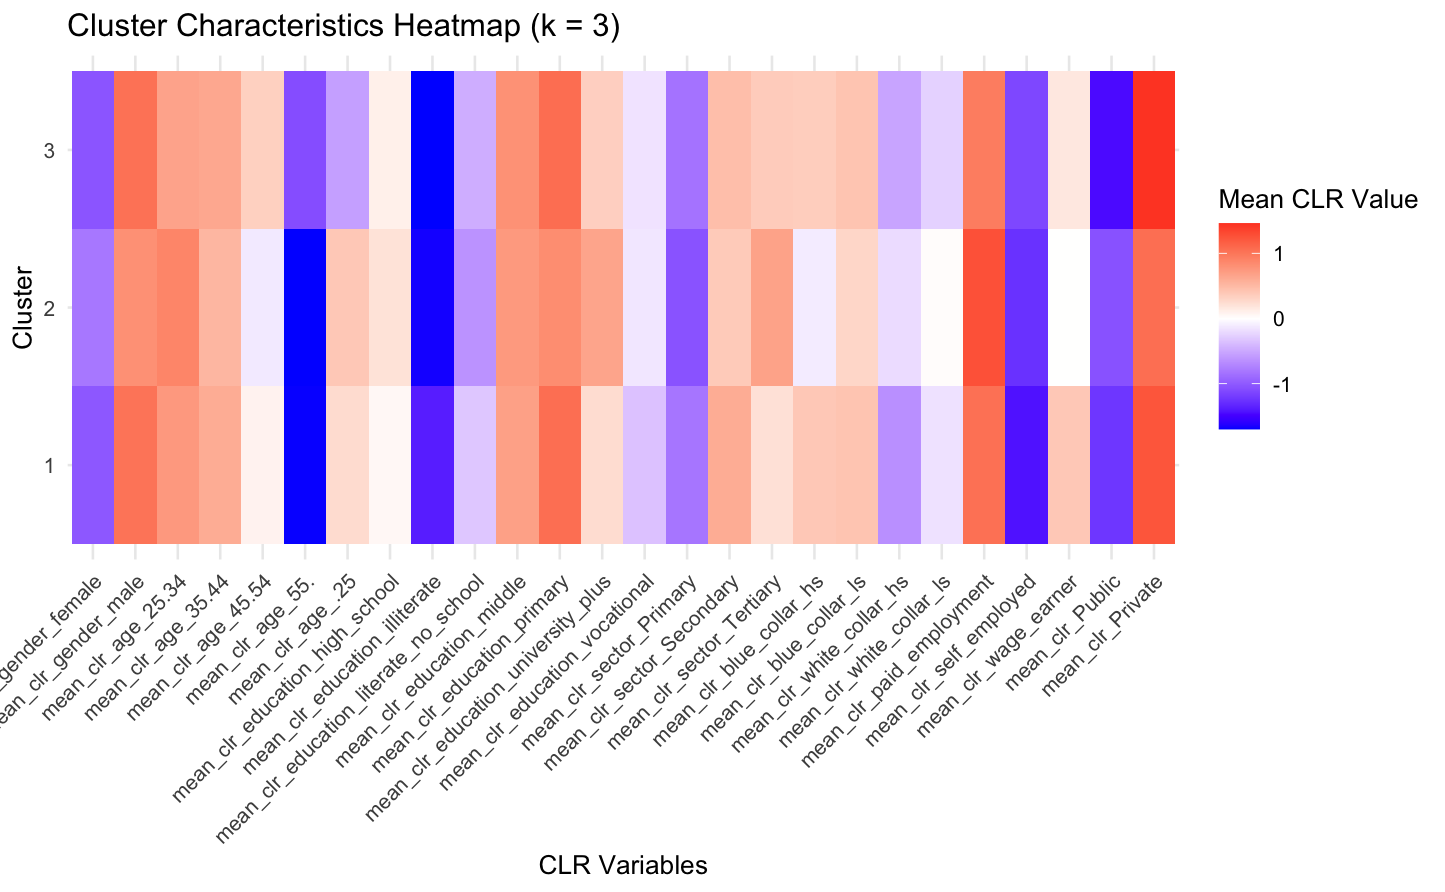
\includegraphics[width=\linewidth]{clr_hier_heatmap.png}
        \caption{Heatmap for k=3, Hierarchical Clustering}
        \label{fig:clr_hier_heatmap}
    \end{minipage}
    \hfill
    \begin{minipage}{0.48\textwidth}
        \centering
        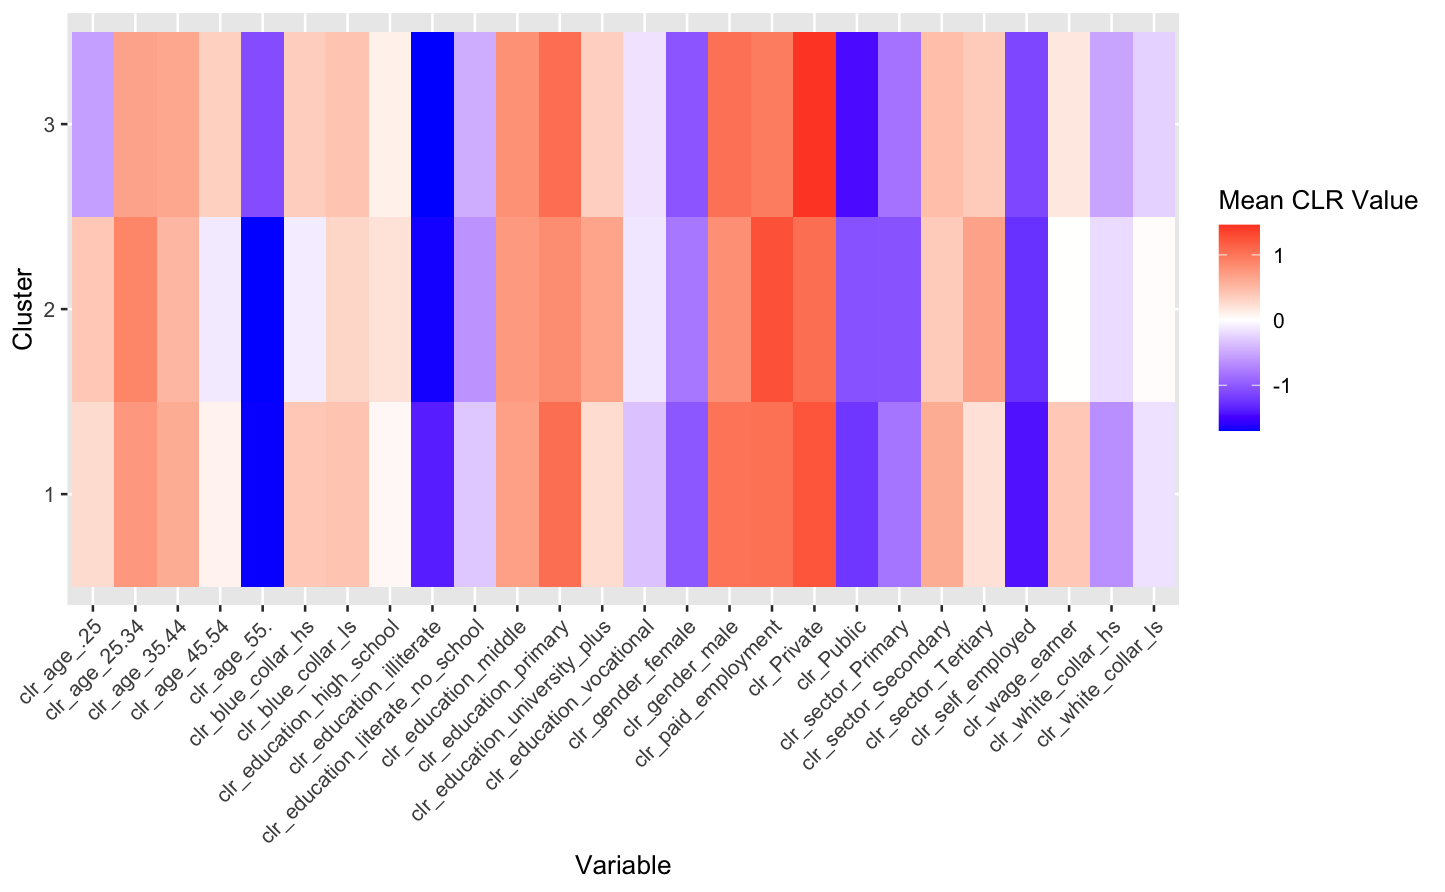
\includegraphics[width=\linewidth]{clr_kmean_heatmap.png}
        \caption{Heatmap for k=3, k-means Clustering}
        \label{fig:clr_kmean_heatmap}
    \end{minipage}
\end{figure}


Heatmaps (Figure ~\ref{fig:clr_hier_heatmap}, ~\ref{fig:clr_kmean_heatmap}) illustrate the mean CLR values for different demographic variables (gender, age groups, education levels, worker types, and sectors) across the three clusters. Cluster 3, which is associated with the general characteristics of the unemployed population under the pandemic, has negative CLR values, signaling an advantage for university graduates, white-collar workers, and public-sector employees. Based on the shifts in clusters over time, it can be inferred that the representation of a group, consisting of males over the age of 55, with vocational education, employed in the private tertiary sector, and primarily self-employed, increased in unemployment.

In general, clustering analysis revealed distinct phases of unemployment dynamics, with significant changes coinciding with key events such as the onset of the pandemic and periods of easing and lockdown restrictions.
These findings imply that the timing and effectiveness of policy interventions may be crucial, suggesting that different phases of the crisis required tailored policy responses. Moreover, the heatmap analysis confirms that the pandemic disproportionately affected certain groups, and the results emphasize the need for differentiated policy approaches to address the specific needs of vulnerable groups during economic crises.

\section{Conclusion}
In this study, a demographic analysis of unemployment through an inspection over COVID-19 in the Turkish labor market has been conducted. The prominent objective and framework of this study has been to assess the demographic shifts in trends in unemployment under COVID-19, by using recent cross-sectional and panel data of TurkStat. To be more specific, a descriptive approach has been employed by tracking individuals and households observed in TurkStat’s SILC Panel Data between 2018 and 2021. Additionally, the study sought to explore the underlying reasons why the pandemic’s effects have been uneven across different segments of the population, which may have significant implications for policy development and social dynamics. To structure the analysis around the COVID-19 timeline, the data has been categorized into two periods: "pre-COVID" (2018-2019) and "post-COVID" (2020-2021). Descriptive plots for each factor and compositional data analysis for their joint effects were constructed. In the middle step, CLR-Transformed variables to be used in clustering analysis were also used for creating descriptive plots with Stringency Index.

In this regard, as has been stressed above in the "Introduction" and "Results" parts, the implications of this study's findings are mixed. It might be because of the fact that:
\begin{itemize}
    \item The data used in this study (SILC Cross-Section, SILC Panel Data of 2018-2021) is different than other related papers in the literature.
    \item The data used in this study has more limitations regarding the labor market. There was no information on post-COVID years and no extended monthly information.
\end{itemize}

Yet there remain some possible implications to deduce. It has been observed that for different age groups, the unemployment rate during the pandemic appears to have increased for individuals above 55, while it may have decreased for those under the age of 25. One possible explanation for this trend has been that older individuals tend to be less skilled and educated, making them more vulnerable to job losses. Additionally, younger people seem to have temporarily exited the labor force, becoming inactive as they waited for the pandemic to subside, a phenomenon frequently discussed in related literature.

In terms of occupational groups, wage earners and self-employed individuals seemed to have experienced higher levels of job losses, as supported by previous findings of \textbf{\cite{aygun2021}}. Furthermore, when controlling for in-group skill levels, high-skilled white-collar workers were found to be the least impacted by the pandemic and the measures taken. This may be attributed to the flexibility and widespread adoption of remote work options during the pandemic.

When unemployment in the labor market was investigated by gender, some disparities were also observed, with a slight increase in unemployment among female workers at the onset of the pandemic, which has been a result that contrasts with the findings of \textbf{\cite{aygun2021}}. 

Additionally, the concept of the \textbf{"shecession"} referring to a gender-specific economic downturn disproportionately affecting women, was not prominently observed in the findings. This result may be attributed to data-related limitations and differences, as well as the fact that the analysis conducted here controlled for individuals consistently participating in the labor force. In addition, individuals with lower levels of education—specifically those who completed primary, middle, or vocational education appear to have been more adversely affected by unemployment during the pandemic, which was also suggested by \textbf{\cite{montenovo2020}}. Lastly, clustering analysis provided valuable insights by presenting multiple perspectives and uncovering more complex interconnections among different demographic groups.

These findings not only contribute to a better understanding of the study's position within the existing literature and highlight certain potential limitations but also offer valuable insights into potential directions for future research in the related field. To the best of available knowledge, this study has broader implications for the existing literature by providing a novel methodological approach through the application of CLR Transformation and Clustering Methods to TurkStat’s SILC Panel Data. By the utilization of this technique and SILC Panel Data, it became relatively easier to track specific individuals in Turkey throughout the years without the pandemic and years after the pandemic. Also, it is believed to provide insightful information about how individuals reacted to ongoing changes in the labor market due to COVID-19. Additionally,
the findings contribute to understanding the heterogeneous economic impact of COVID-19 across different demographic groups in Turkey, offering a framework that can be applied to similar datasets in other contexts. However, certain limitations must certainly be acknowledged, such as potential biases because of data limitations and the exclusion of informal sector dynamics, which may have influenced the observed trends in this paper. Additionally, future research could build upon this work by incorporating longitudinal data from a broader time frame, exploring additional variables like health outcomes and access to social welfare, or applying alternative statistical methods to further improve the robustness of the findings. In addition, expanding the analysis to cross-country comparisons may also provide further insights into how different policy responses influenced economic outcomes across diverse populations. 

Lastly, understanding the variations in unemployment among different demographic groups in Turkey, along with the underlying causes and effects of these disparities, serves as a foundation for fostering a more inclusive society. In this context, the present study builds upon previous research by introducing a distinct perspective and methodology, utilizing data that differs from that used in earlier analyses of the unemployment effects of COVID-19 on the Turkish labor force. Previous studies highlighted inequalities across various sub-groups and identified contributing factors, thus laying the groundwork for future research and policy development. It is anticipated that this study will contribute to the related literature similarly by raising new policy questions and inspiring further qualitative and quantitative research regarding the unemployment impacts of COVID-19 in Turkey.












\bibliography{references}


\appendix
\section{Appendix}

An online appendix can also be found for detailed background work in R as well as other expected files for the course in \href{https://github.com/zebozoklu/EC48K}{this GitHub repository}. 

\subsection{Plot for the Decomposition} \label{appendix:decomposition}

\begin{figure} [H]
    \centering
    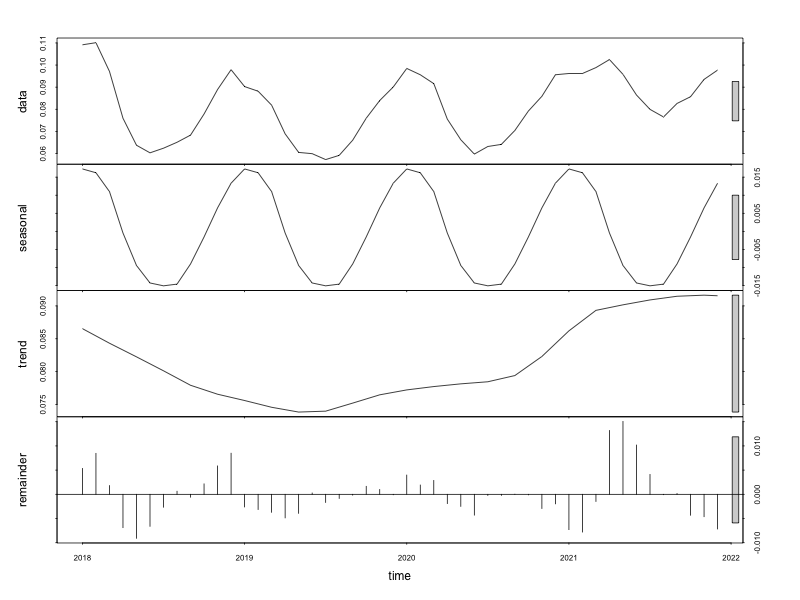
\includegraphics[width=0.8\linewidth]{stl_decomposition_plot.png}
    \caption{Decomposition of Unemployment for Trend}
    \label{fig:stl_decomposition_plot}
\end{figure}

\subsection{Descriptive Plots}
\label{appendix:descriptive-plots}

\begin{figure} [H]
    \centering
    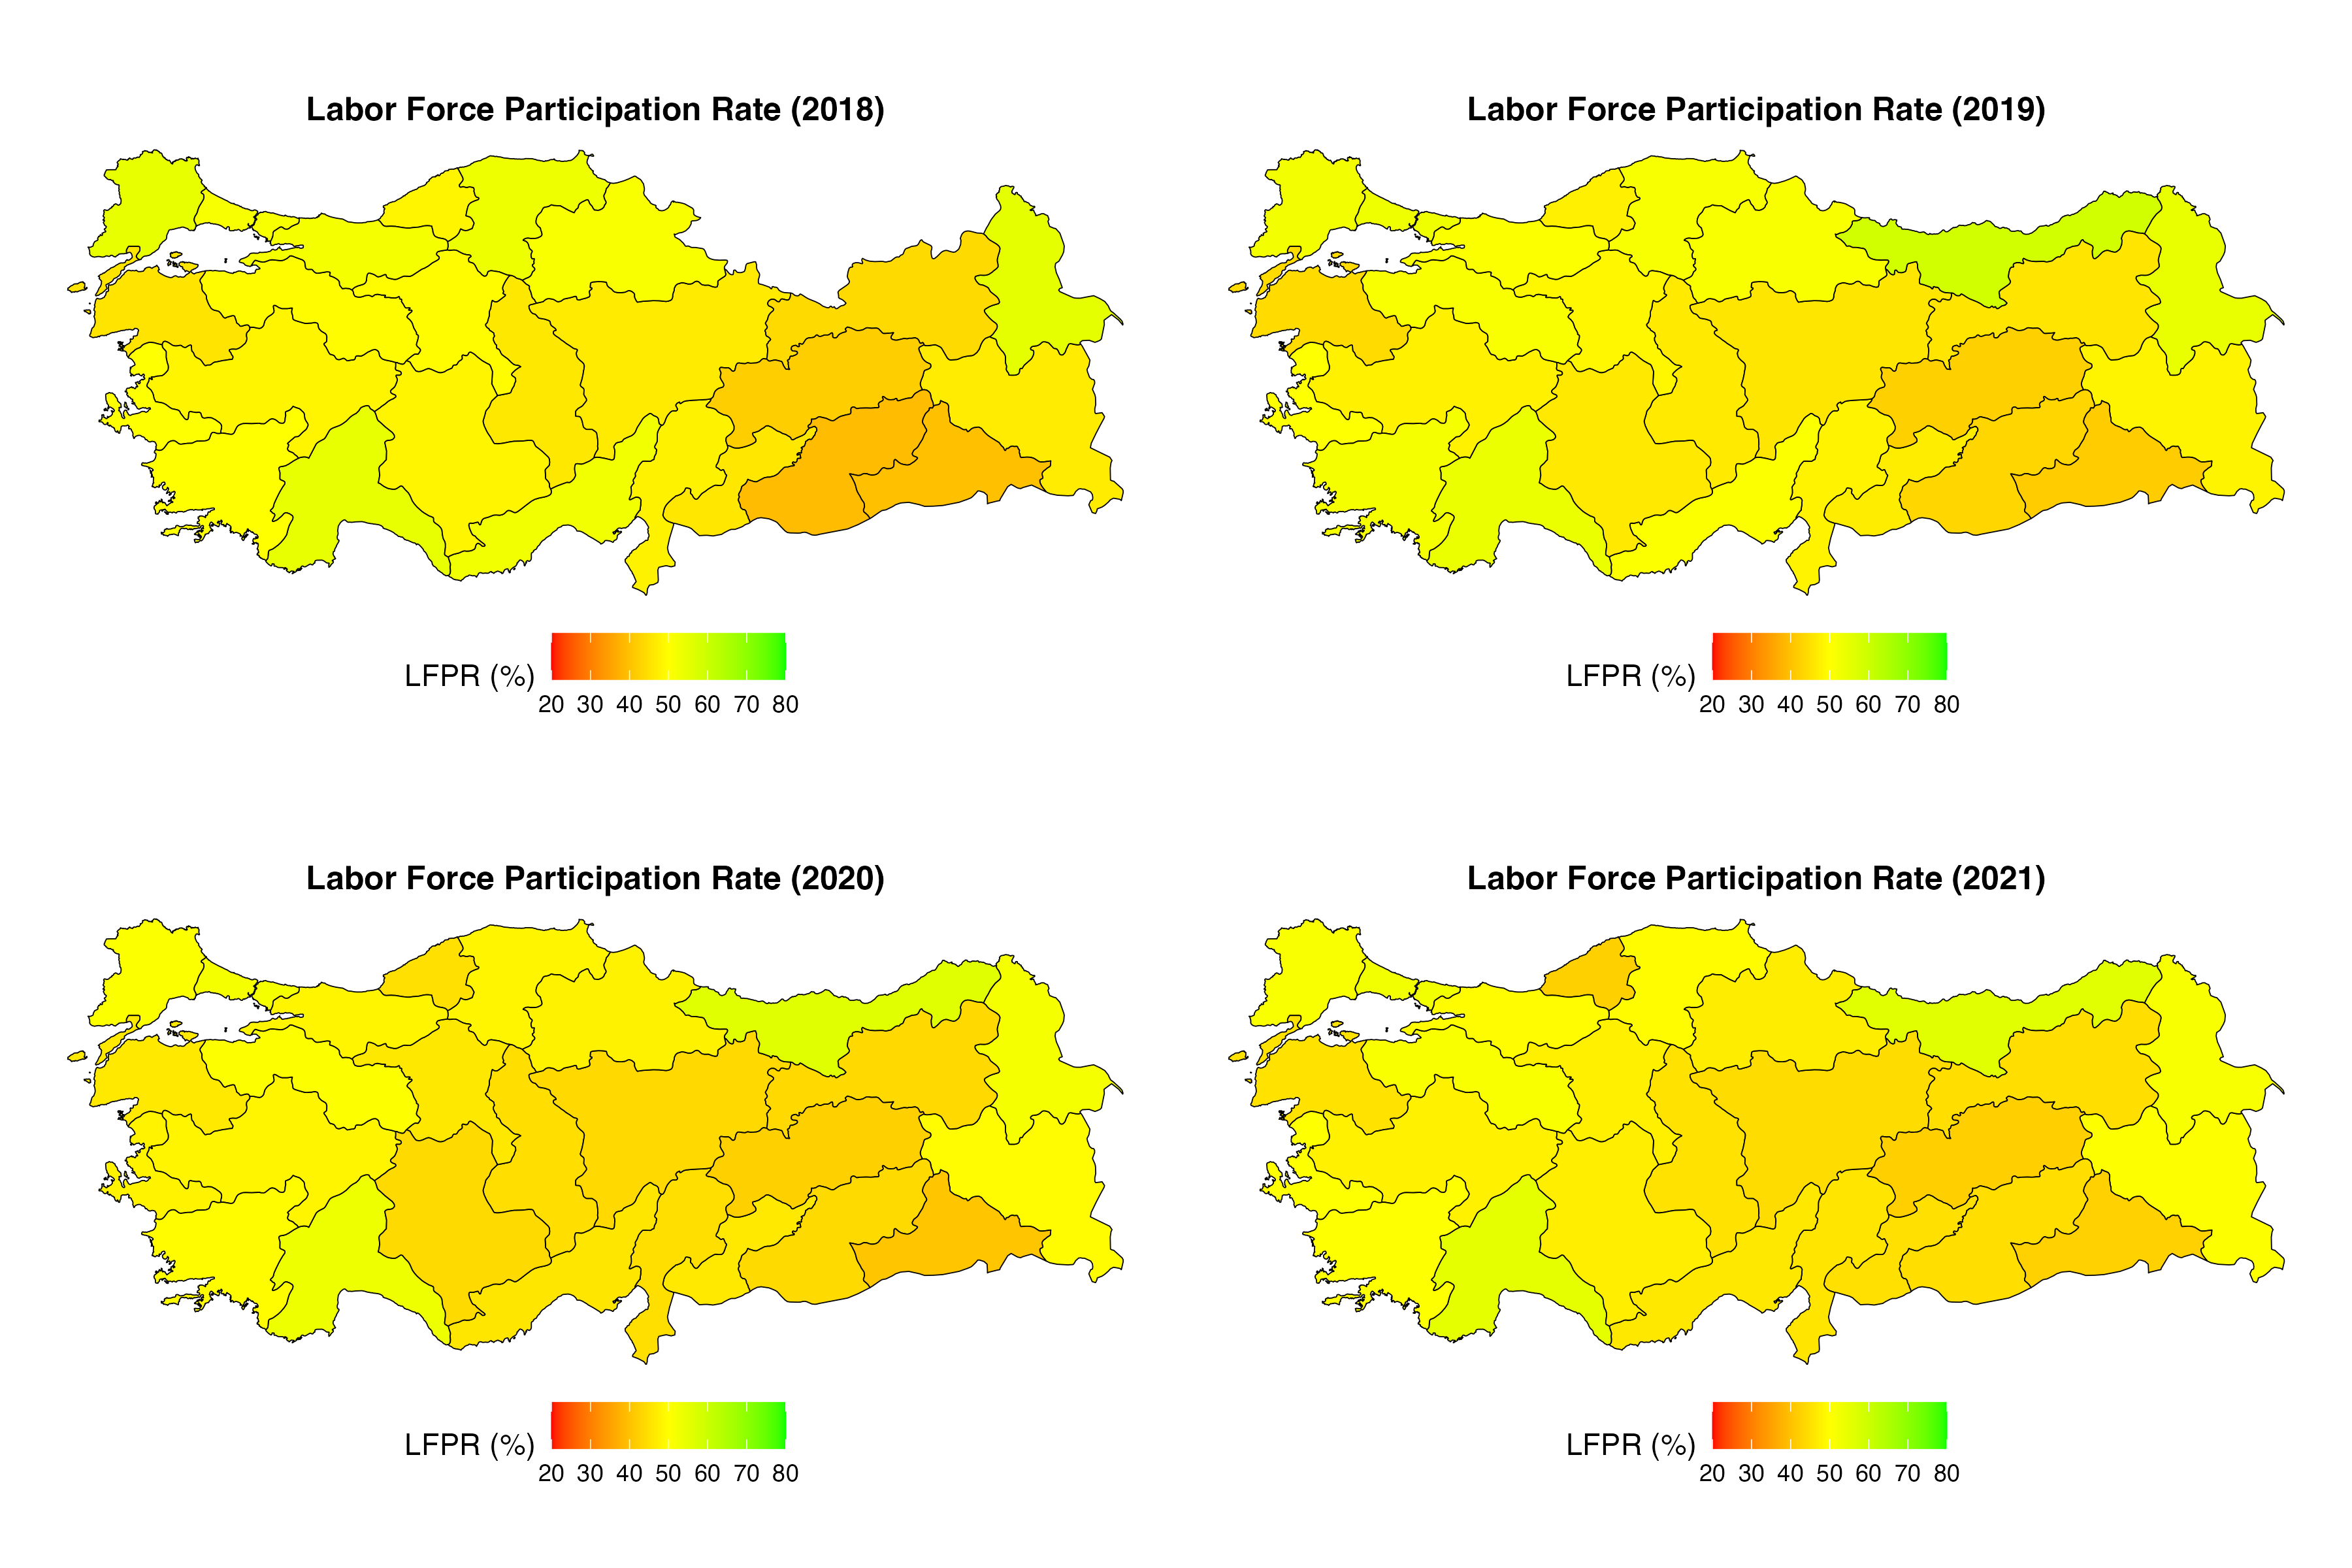
\includegraphics[width=0.8\linewidth]{lfpr_maps_2018_2021.png}
    \caption{Labor Force Participation Rates}
    \label{fig:lfpr_maps_2018_2021}
\end{figure}

\begin{figure} [H]
    \centering
    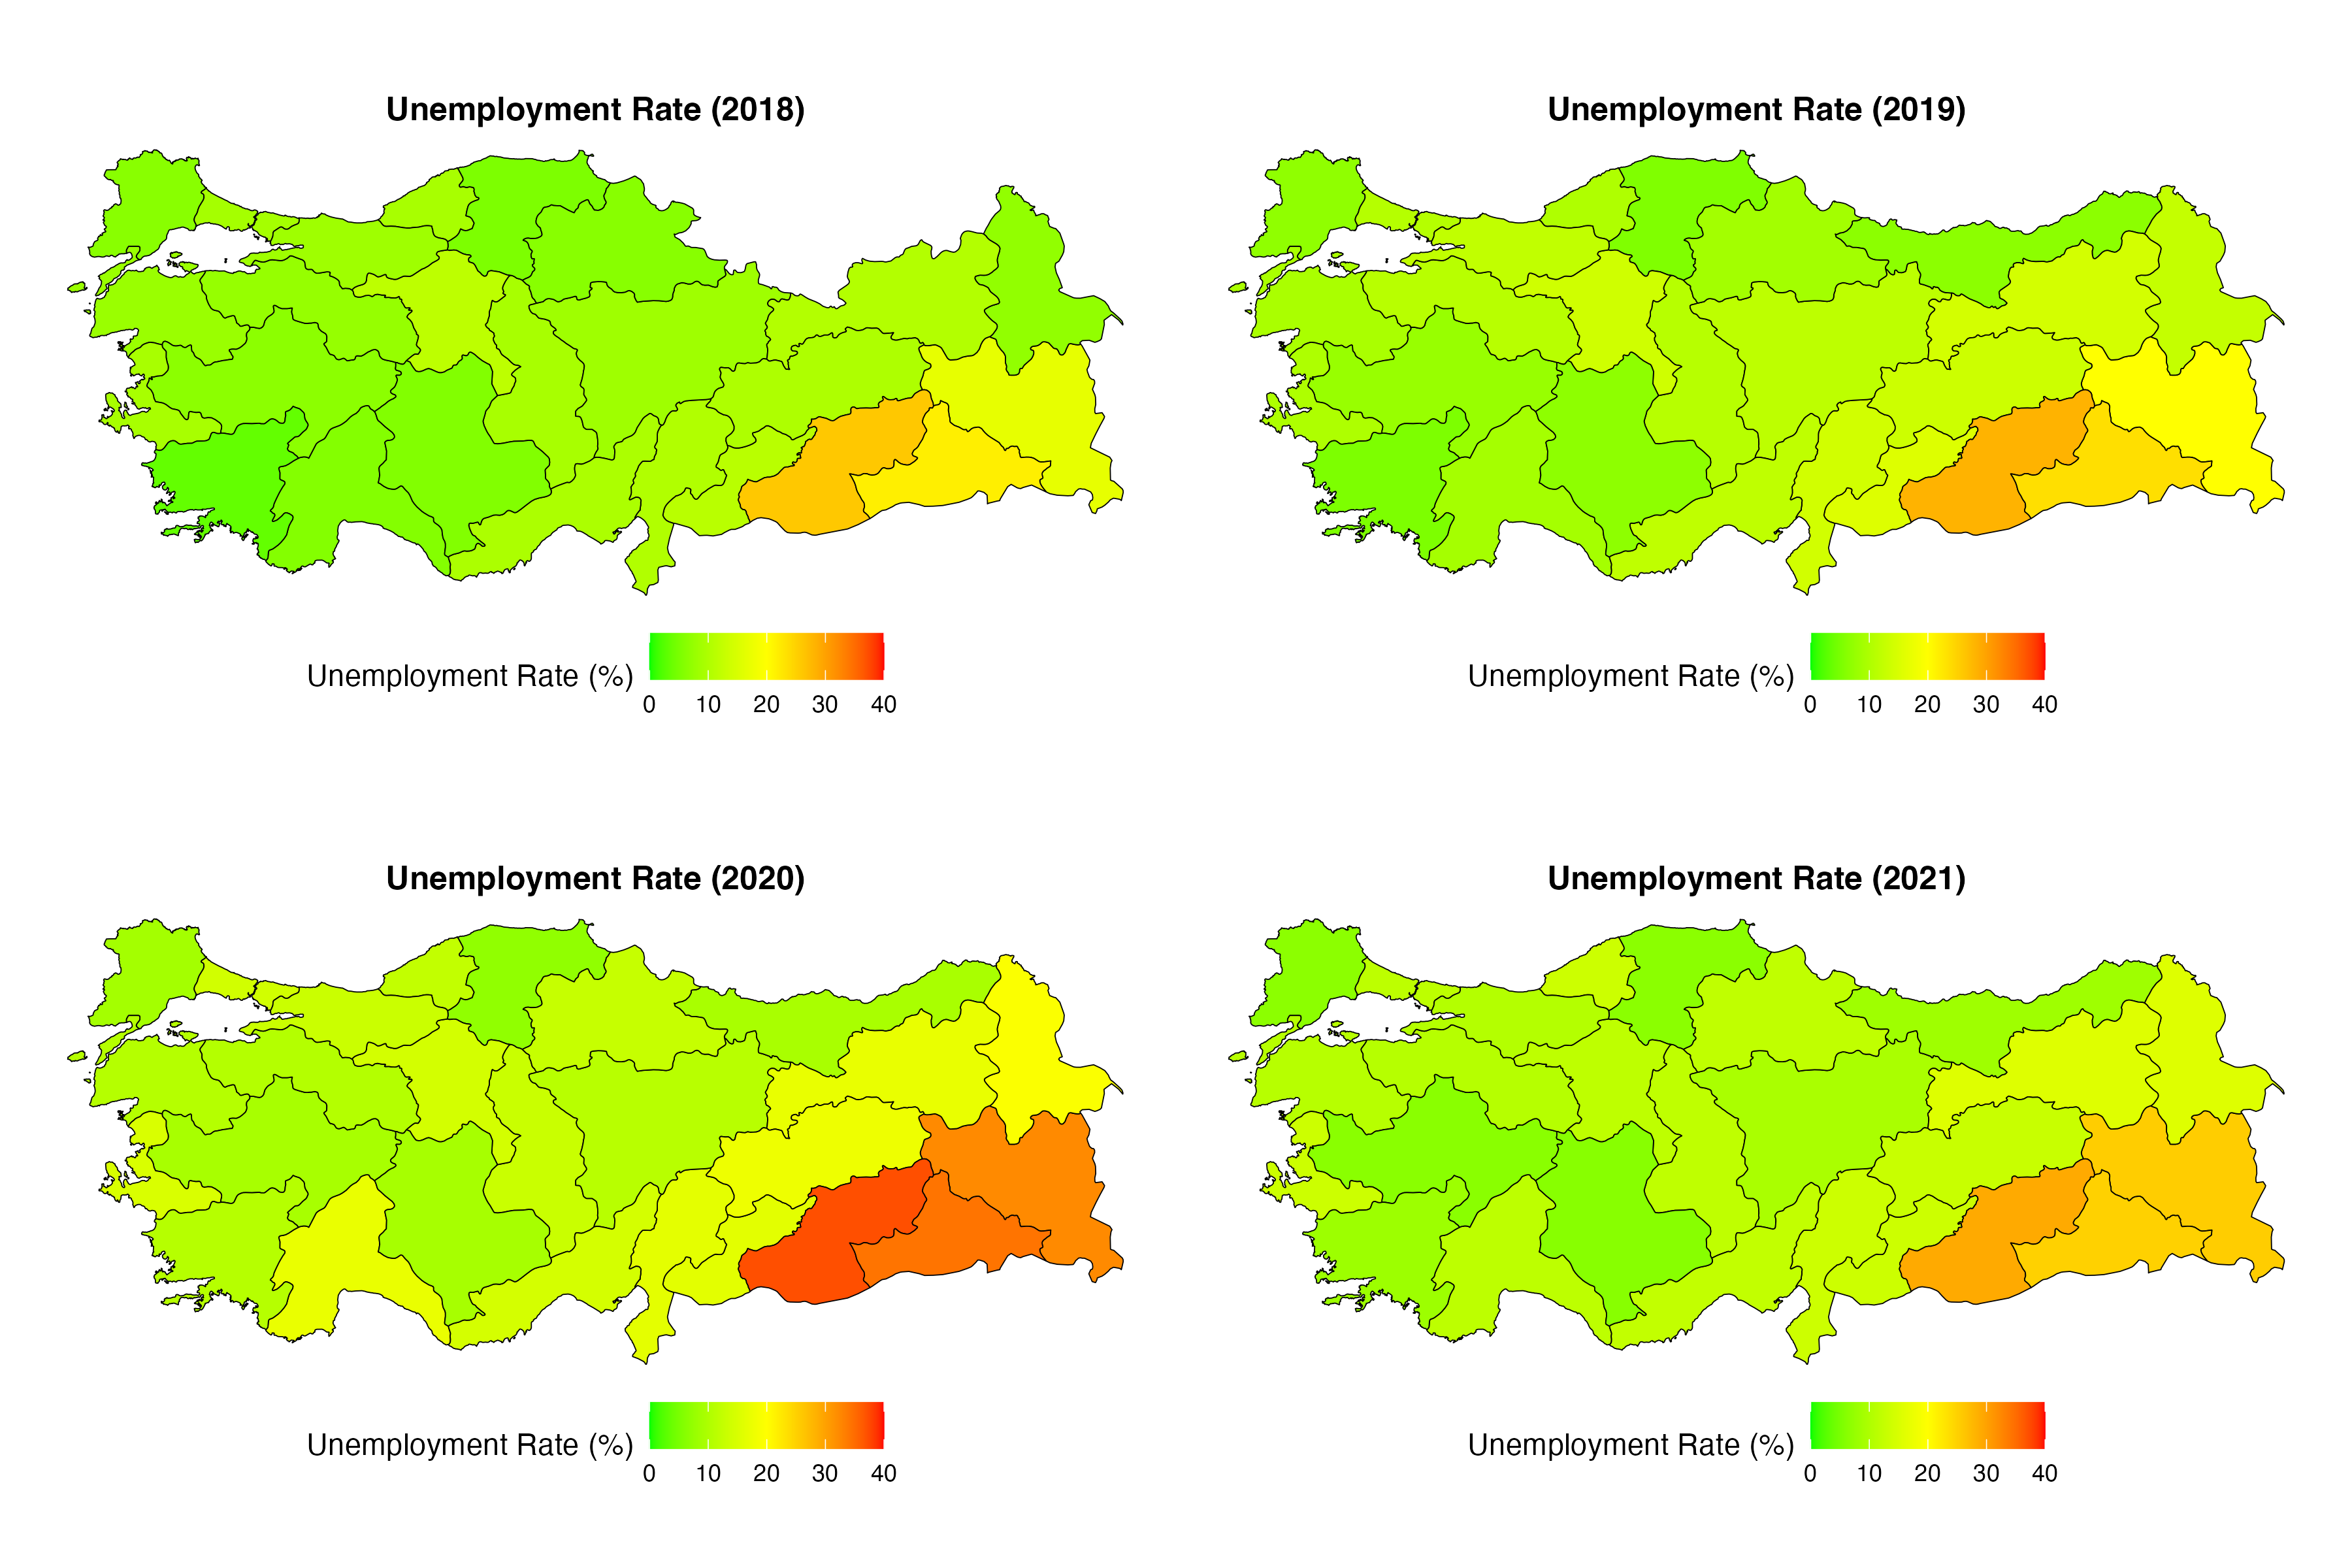
\includegraphics[width=0.8\linewidth]{unemployment_maps_2018_2021.png}
    \caption{Unemployment Rates}
    \label{fig:unemployment_maps_2018_2021}
\end{figure}

\begin{figure} [H]
    \centering
    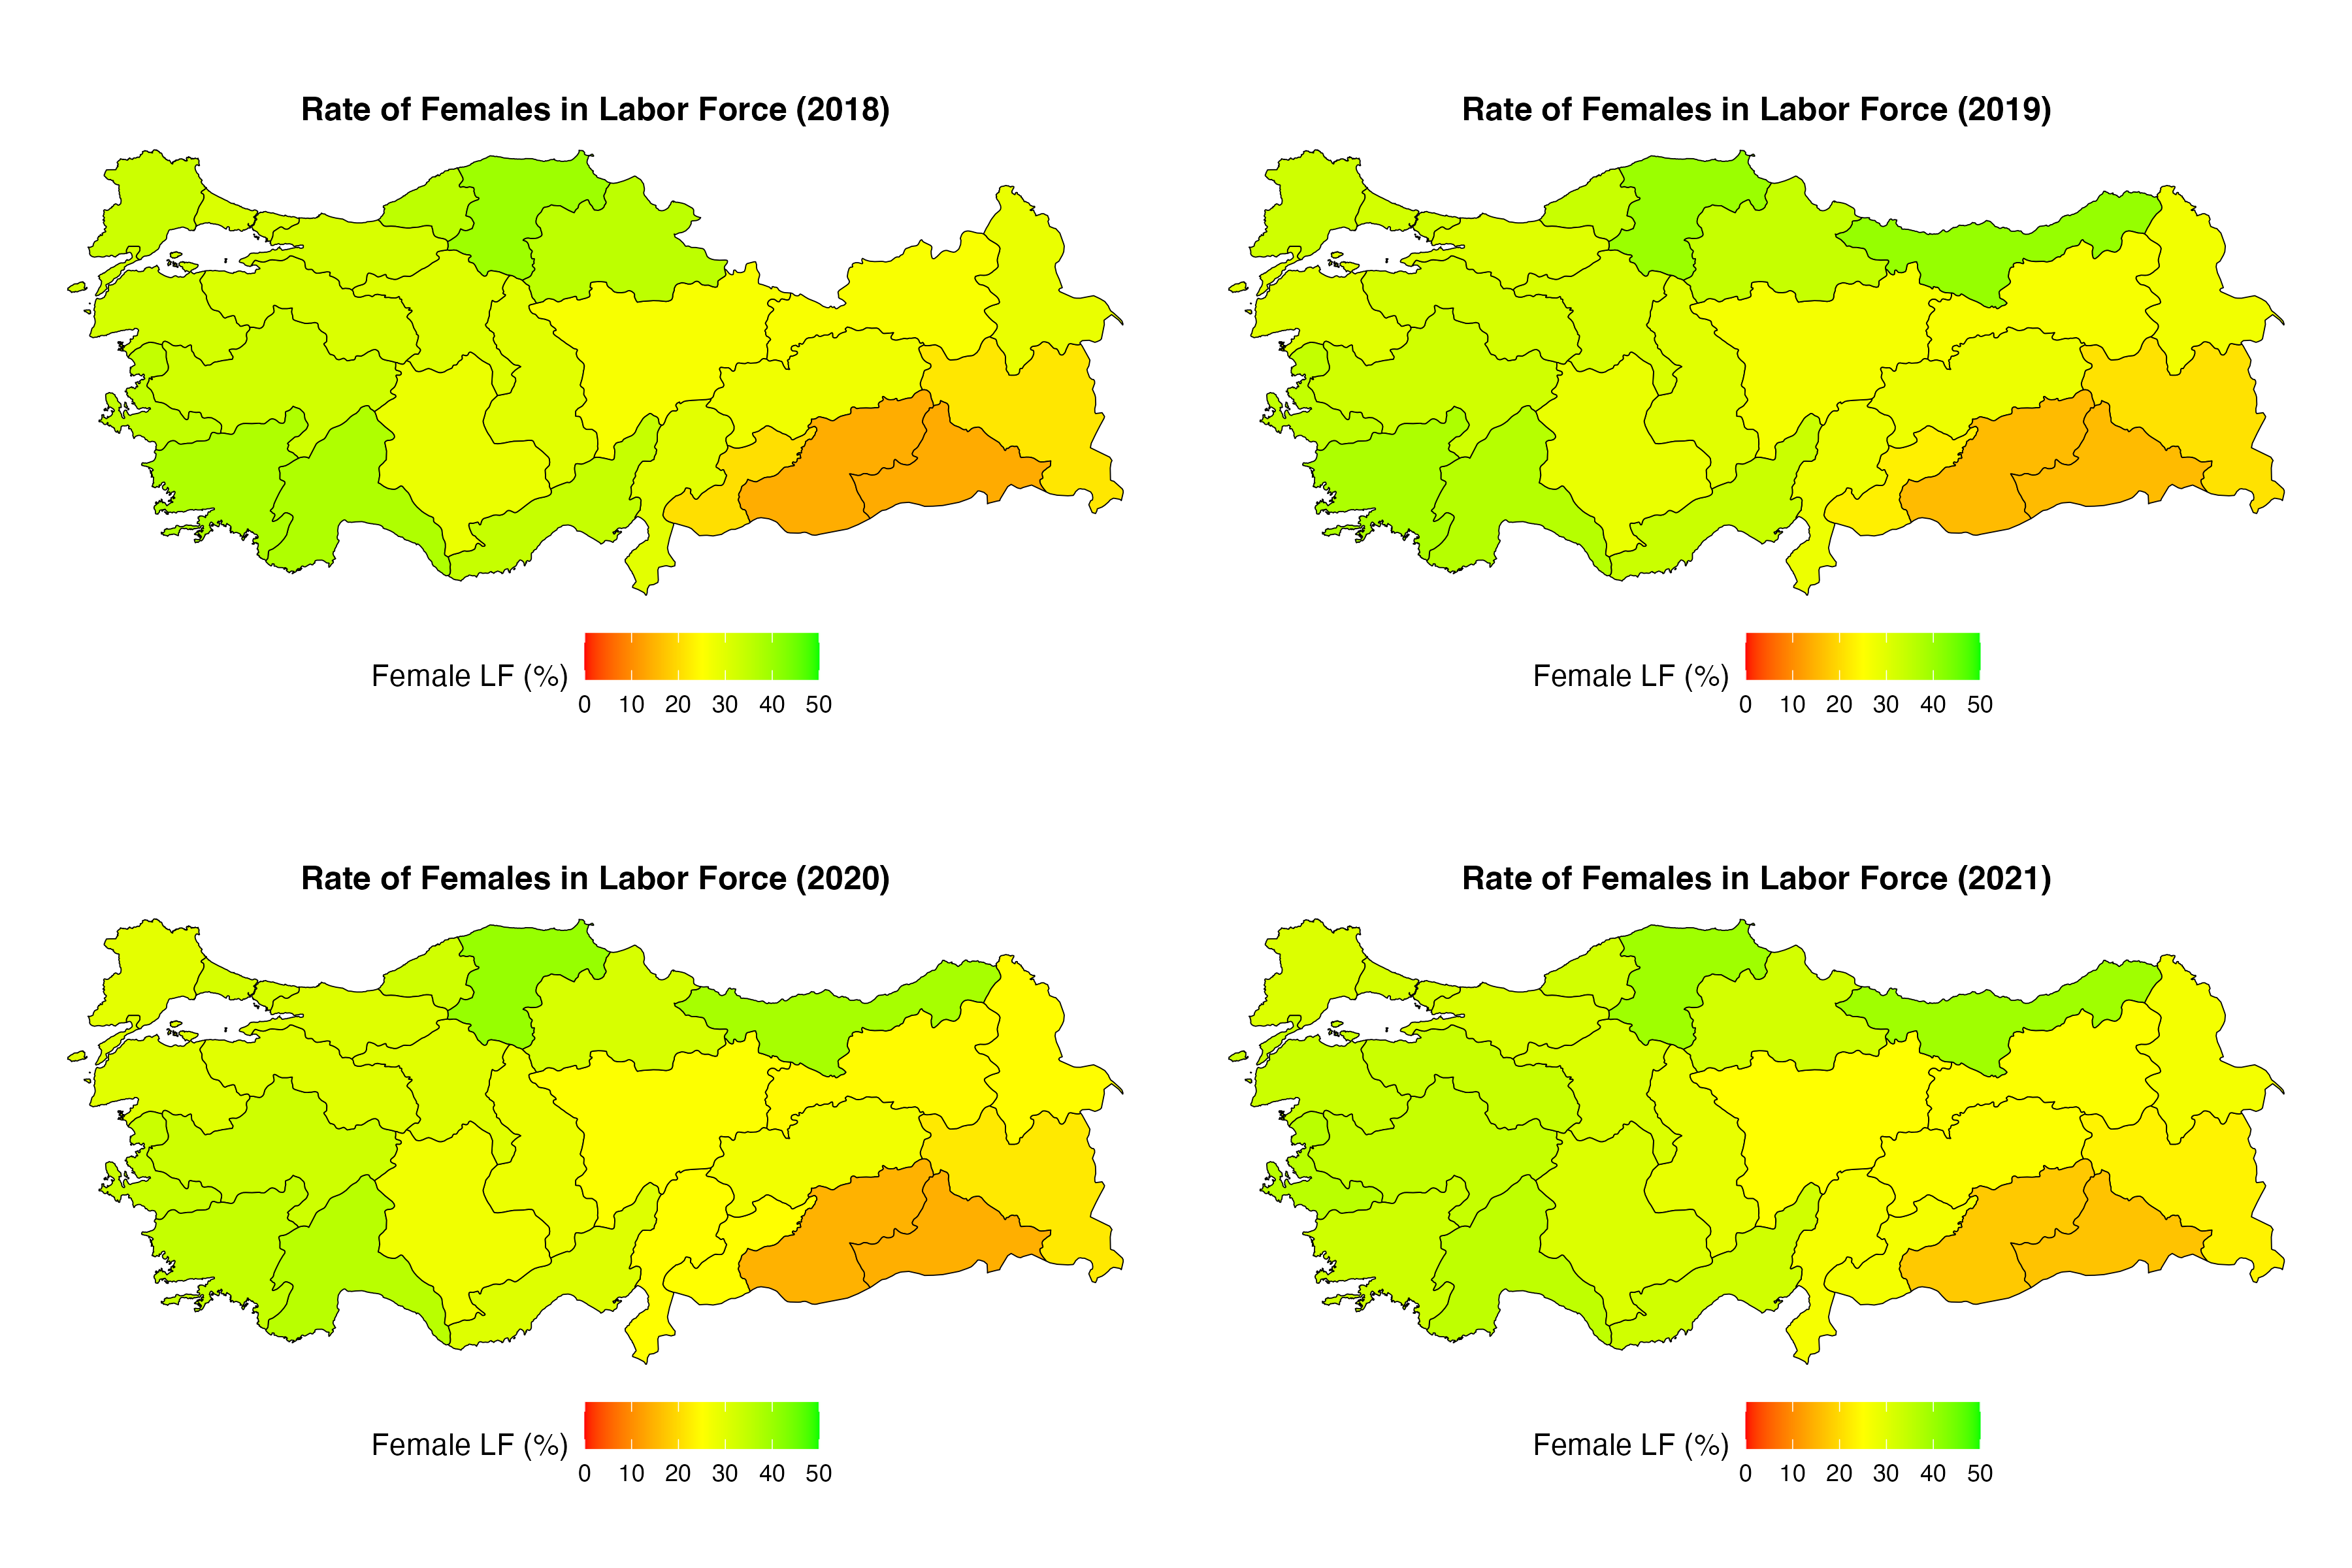
\includegraphics[width=0.8\linewidth]{female_lf_maps_2018_2021.png}
    \caption{Share of Females in the Labor Force}
    \label{fig:female_lf_maps_2018_2021}
\end{figure}

\begin{figure} [H]
    \centering
    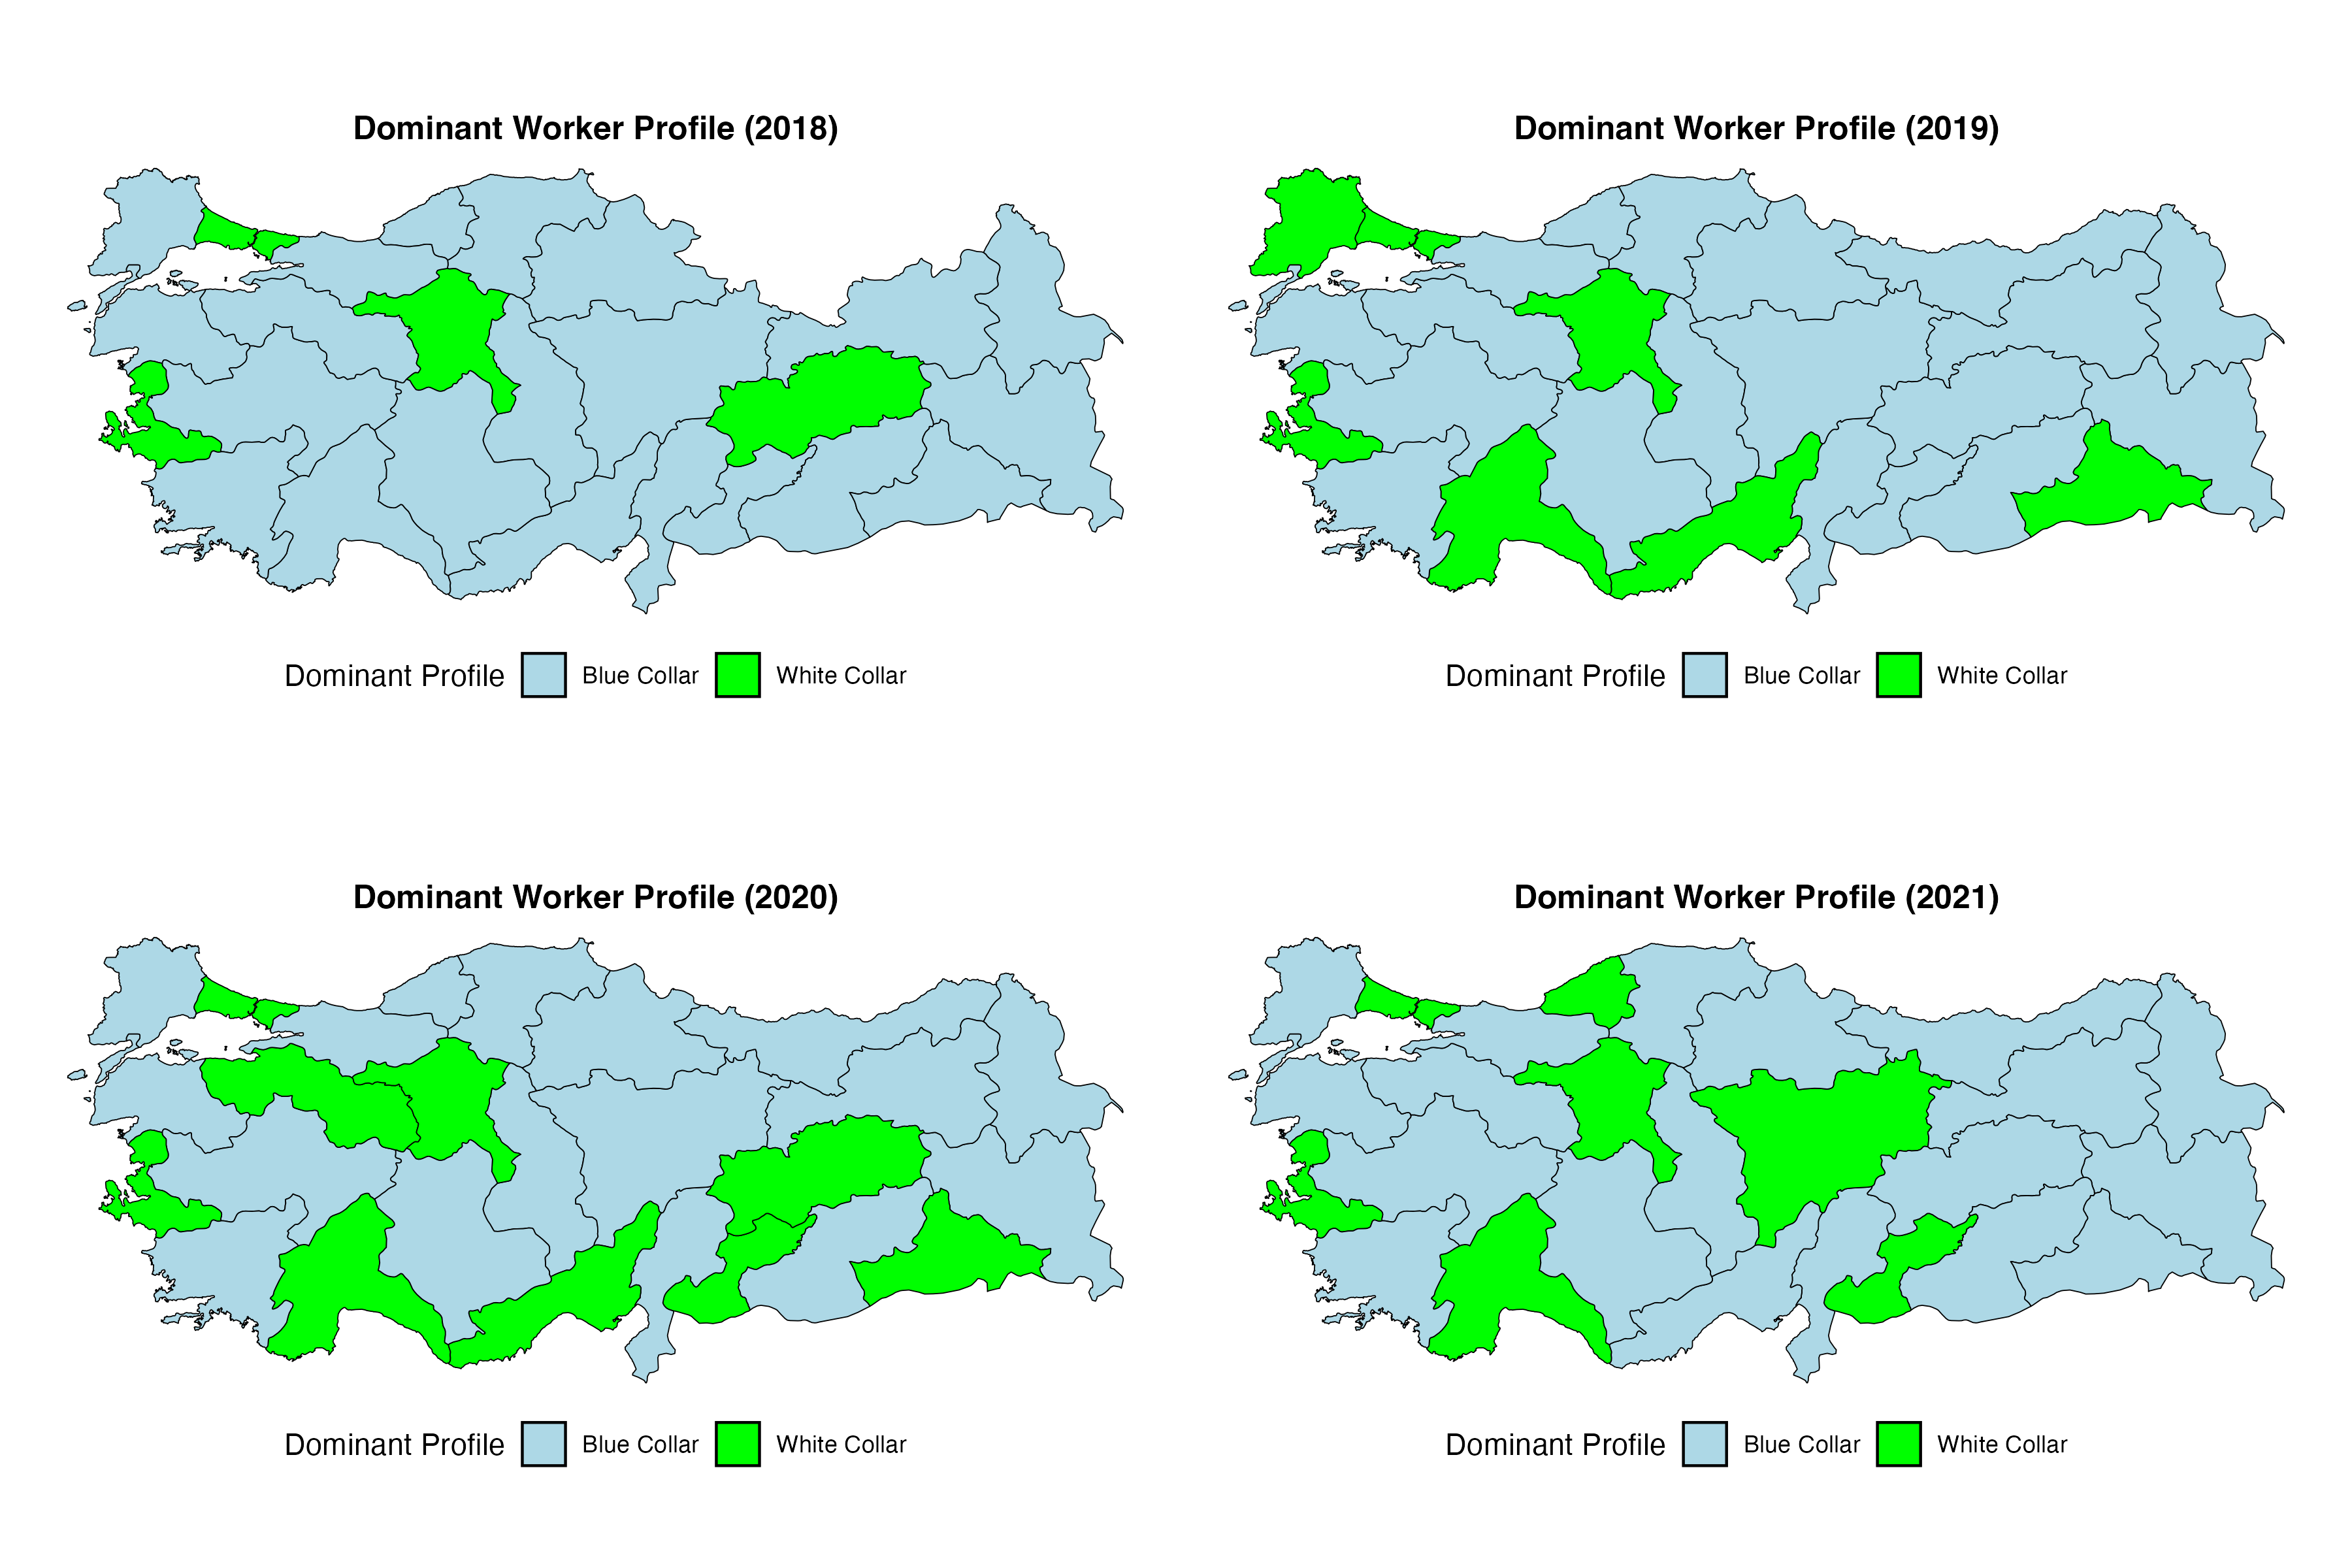
\includegraphics[width=0.8\linewidth]{dominant_worker_profiles_2018_2021.png}
    \caption{Dominant Worker Profiles}
    \label{fig:dominant_worker_profiles_2018_2021}
\end{figure}

\begin{figure} [H]
        \centering
        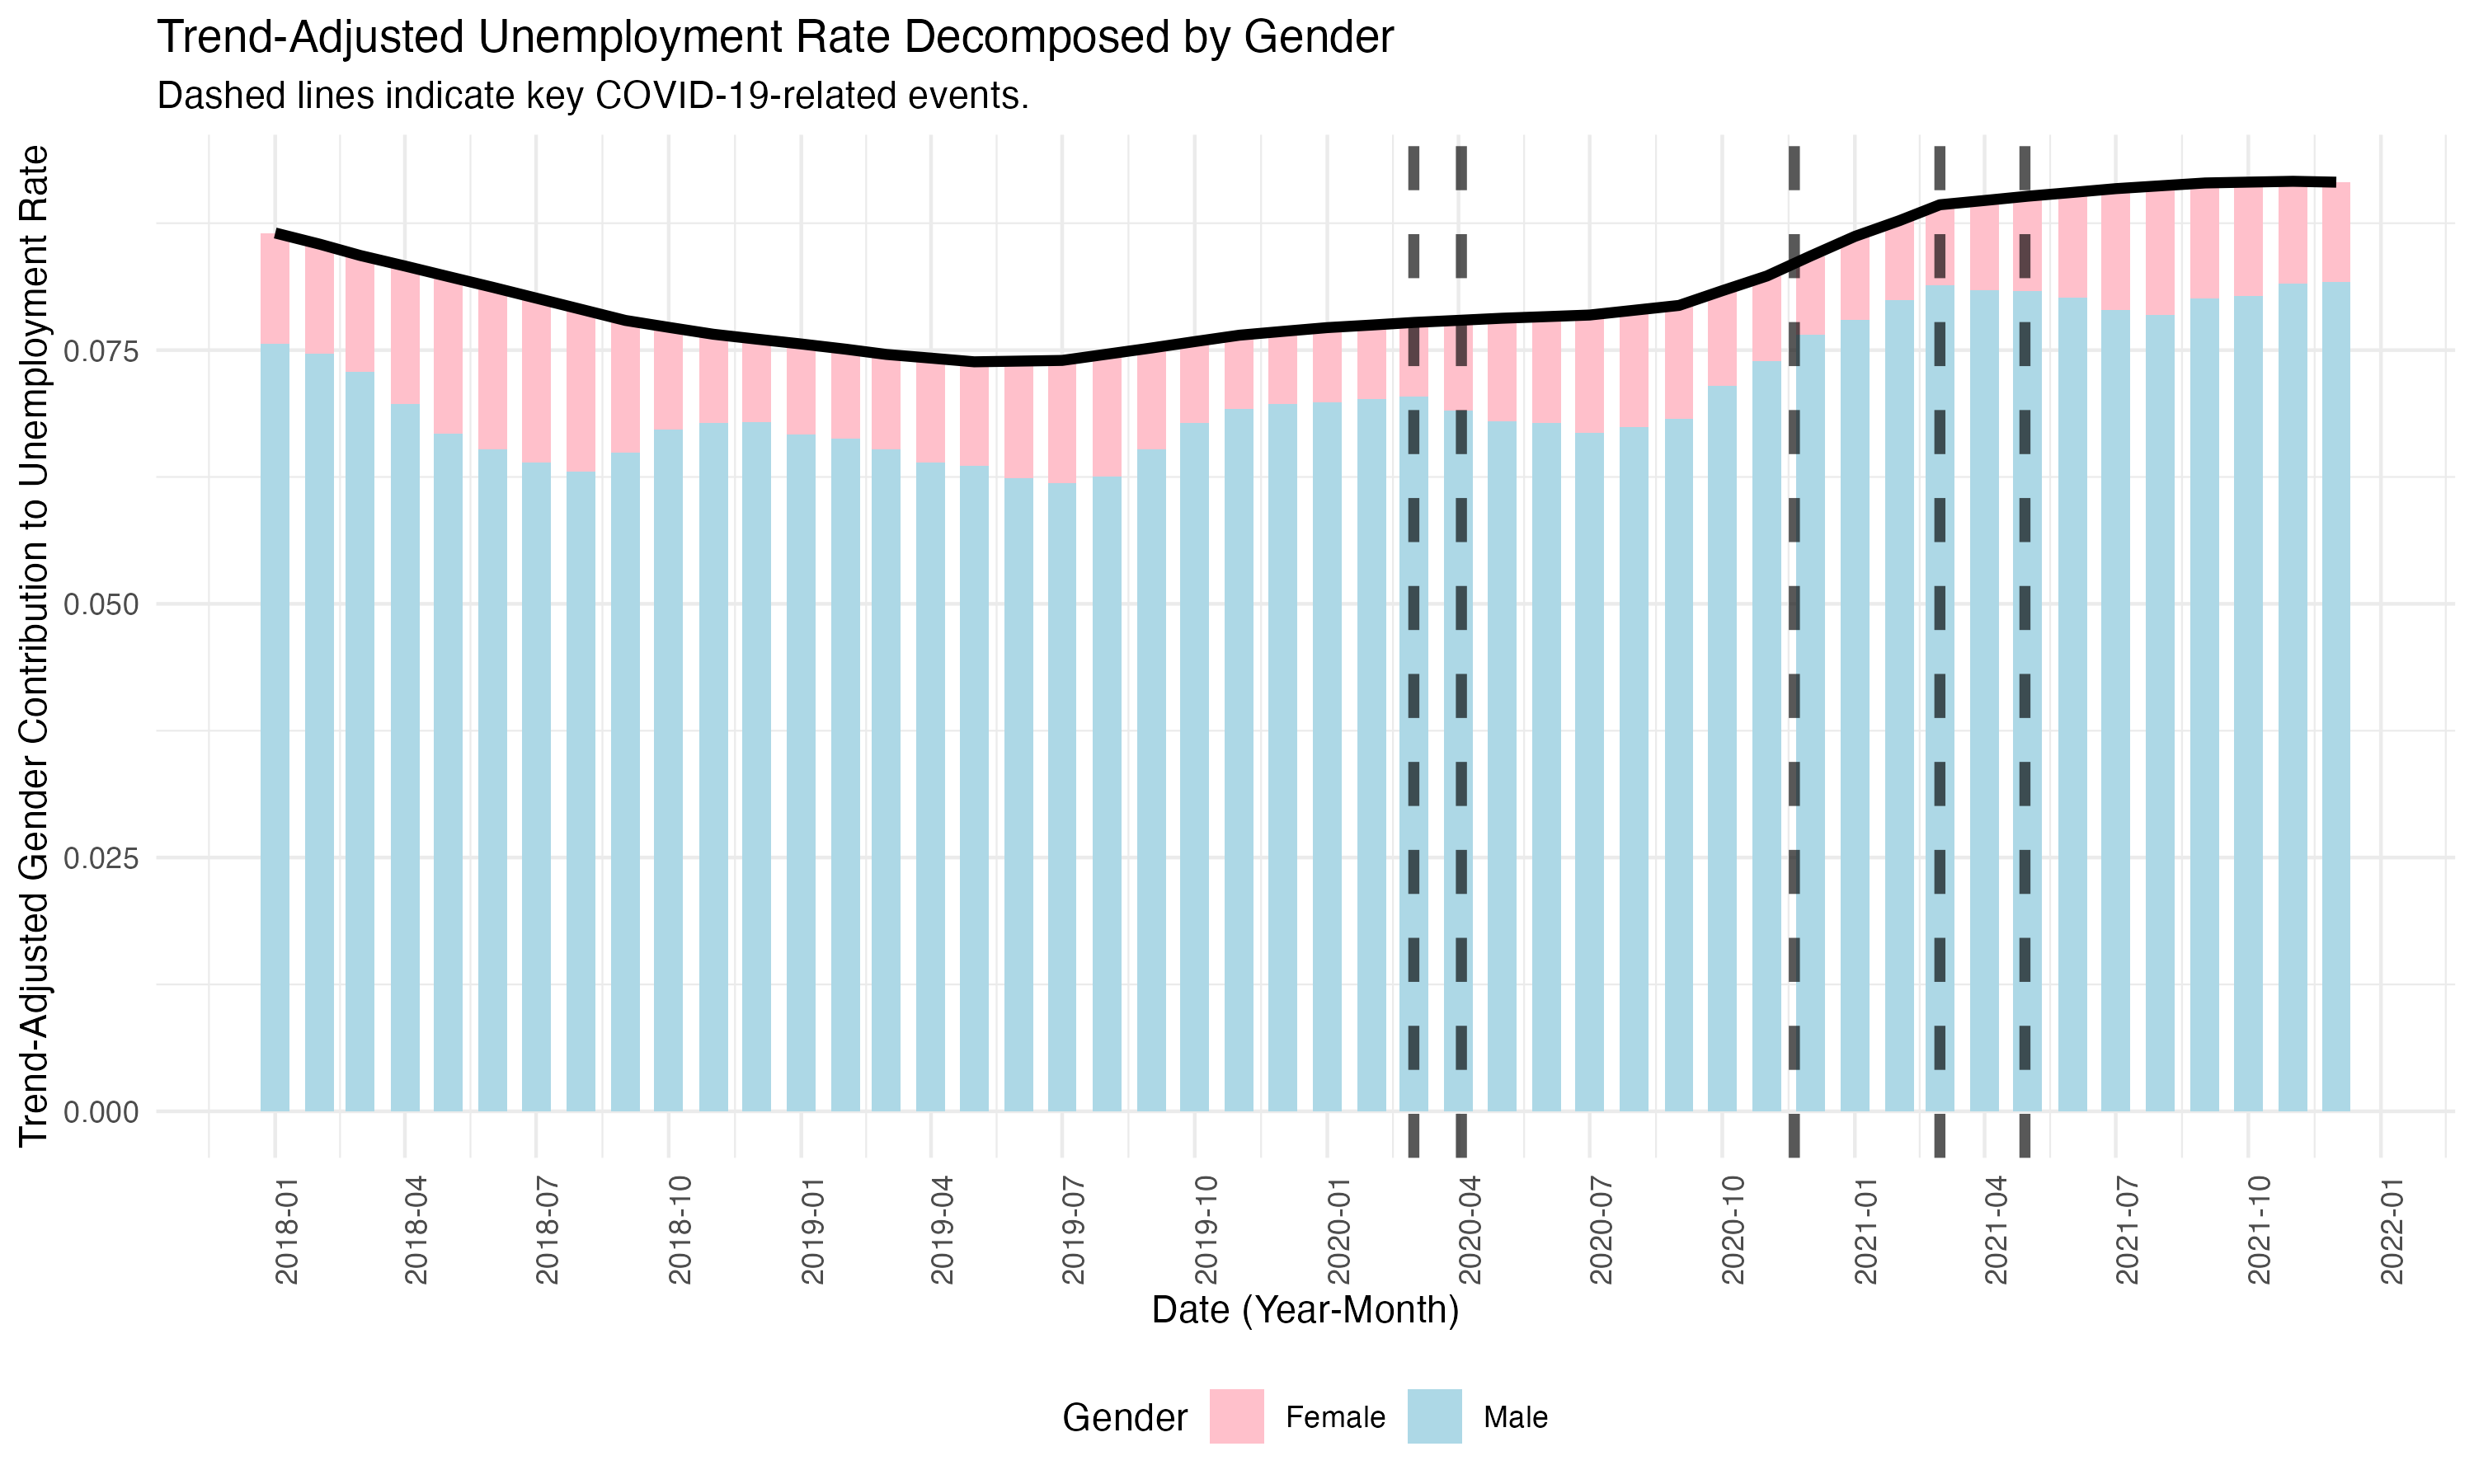
\includegraphics[width=0.8\linewidth]{gender_adjusted_plot.png}
        \caption{Trend Adjusted Unemployment - Gender Decomposition}
        \label{fig:trend_adj_gender}
\end{figure}

\begin{figure} [H]
        \centering
        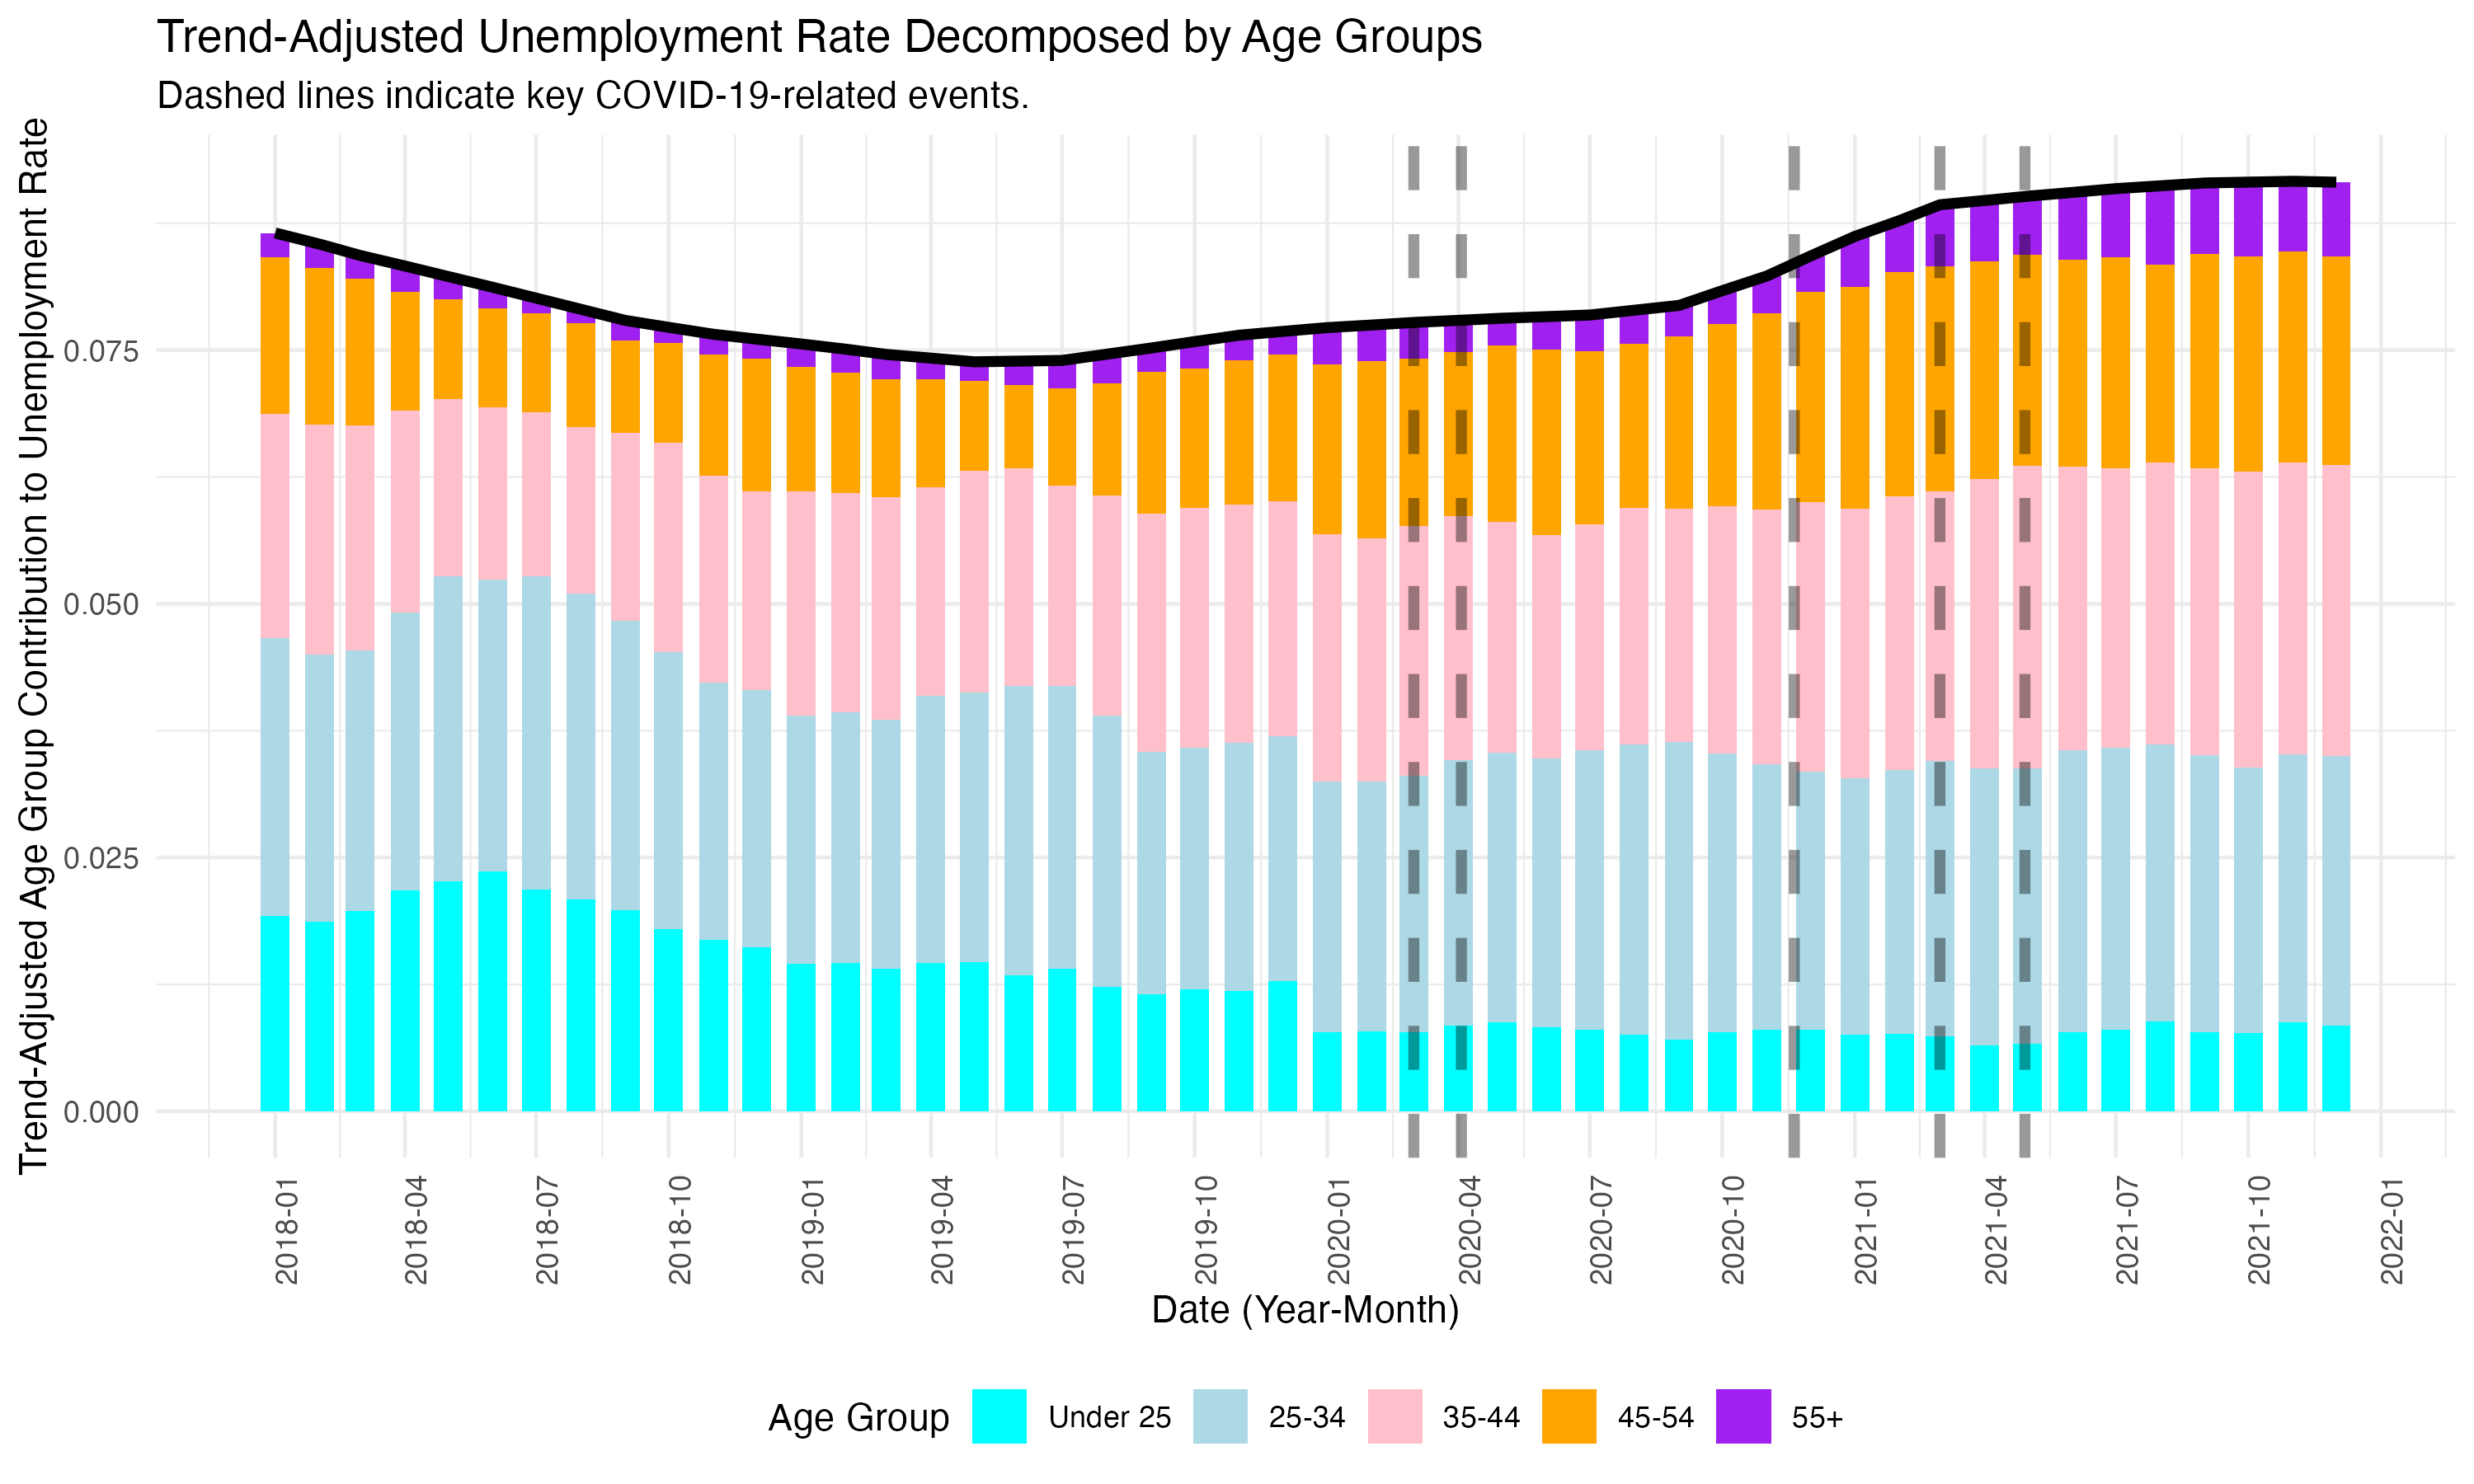
\includegraphics[width=0.8\linewidth]{age_adjusted_plot.png}
        \caption{Trend Adjusted Unemployment - Age Groups}
        \label{fig:trend_adj_age}
\end{figure}

    \begin{figure} [H]
            \centering
            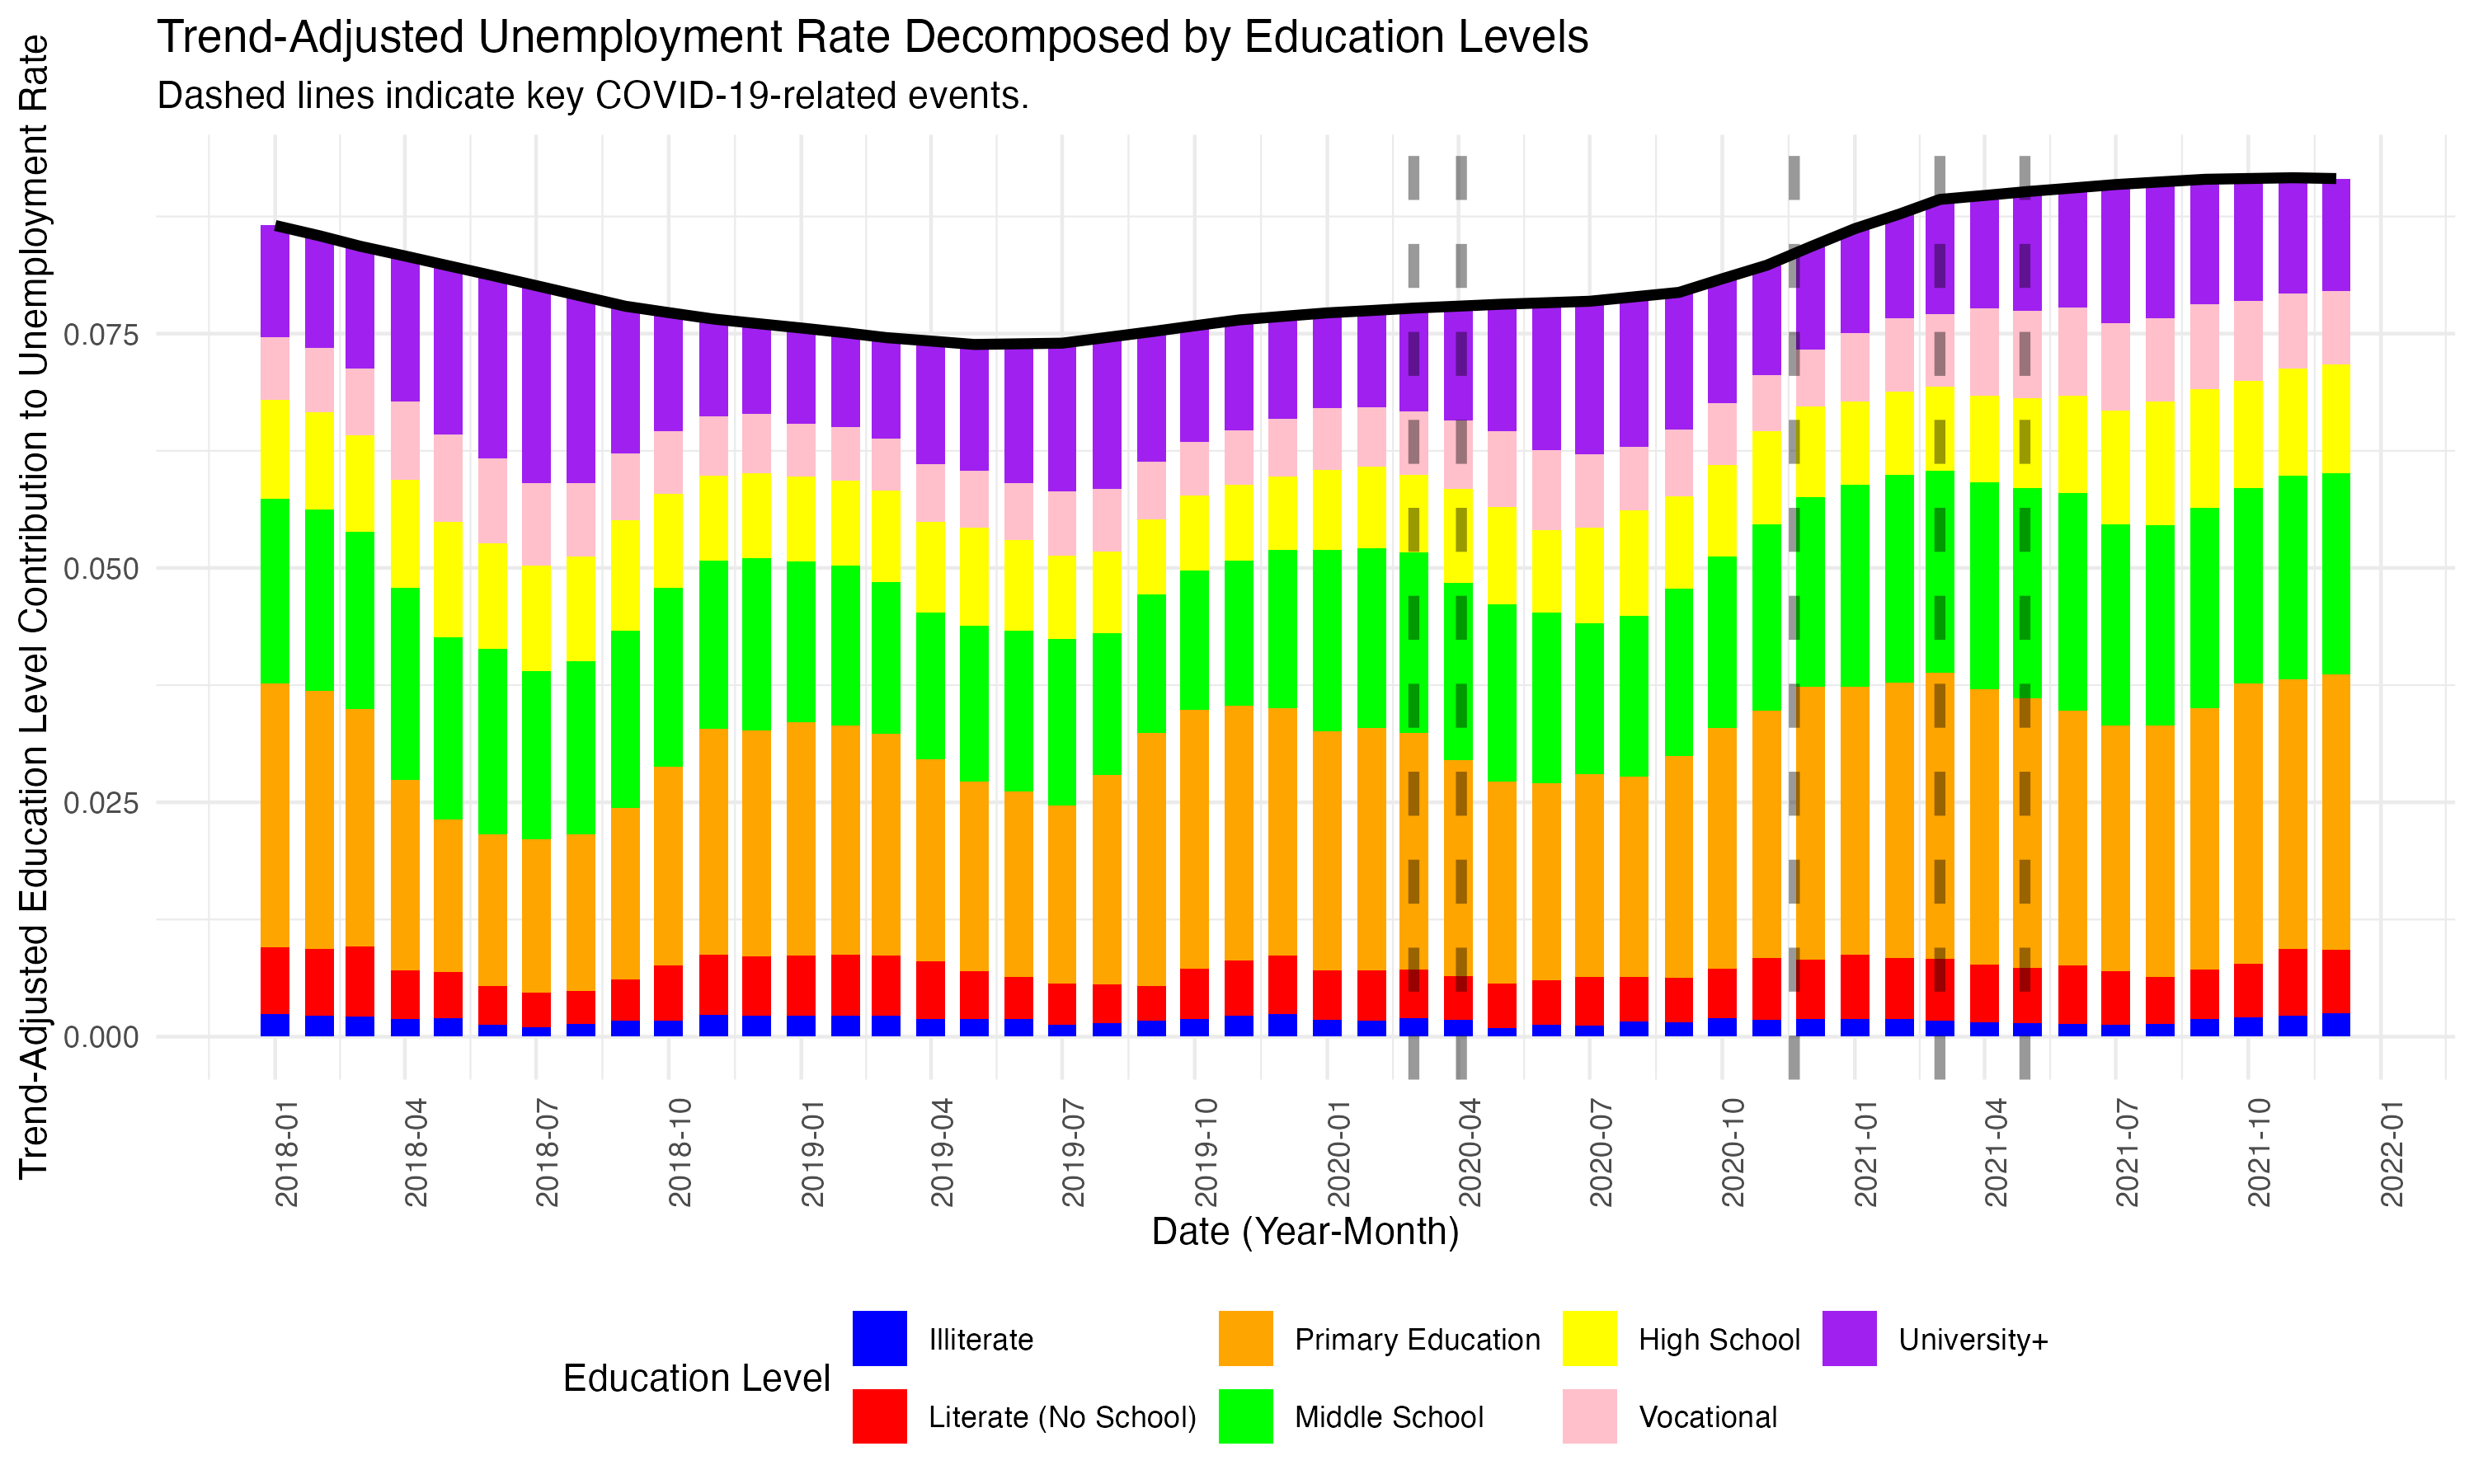
\includegraphics[width=0.8\linewidth]{education_adjusted_plot.png}
            \caption{Trend Adjusted Unemployment - Education Levels}
            \label{fig:trend_adj_educ}
    \end{figure}

    \begin{figure} [H]
        \centering
        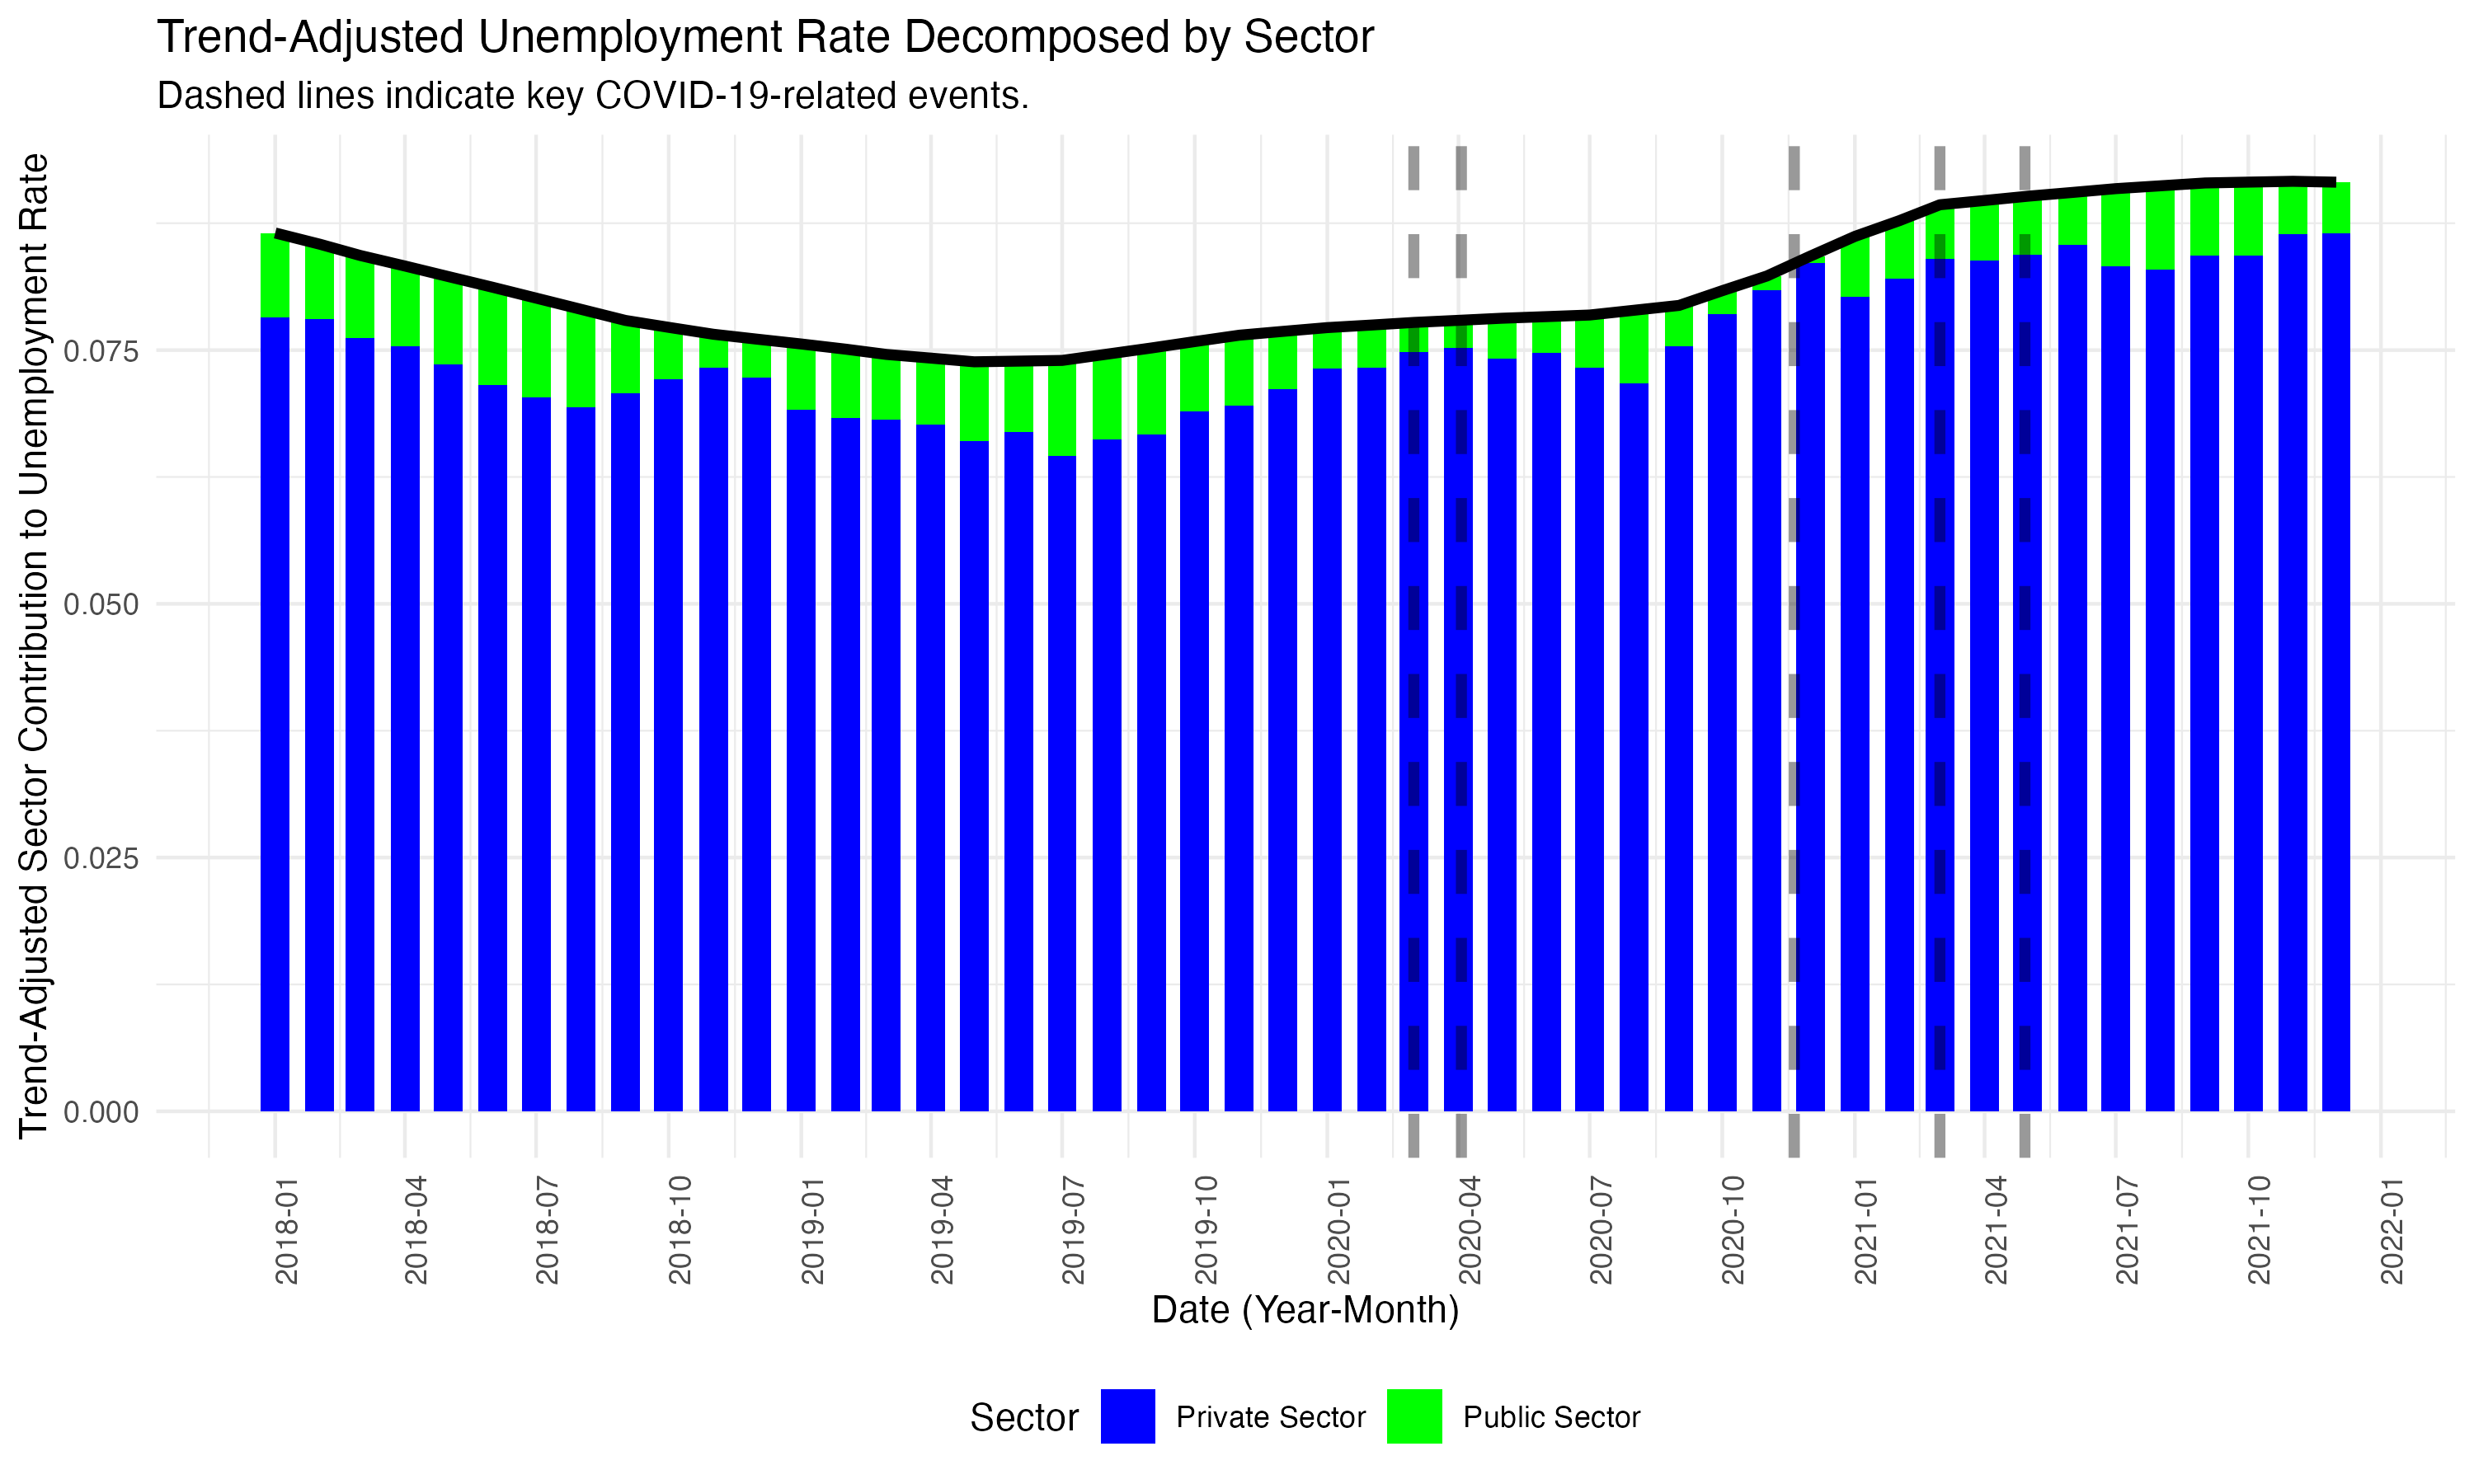
\includegraphics[width=0.8\linewidth]{sector_adjusted_plot.png}
        \caption{Trend Adjusted Unemployment - Establishment Decomposition}
        \label{fig:trend_adj_pubpriv}
    \end{figure}

    \begin{figure} [H]
        \centering
        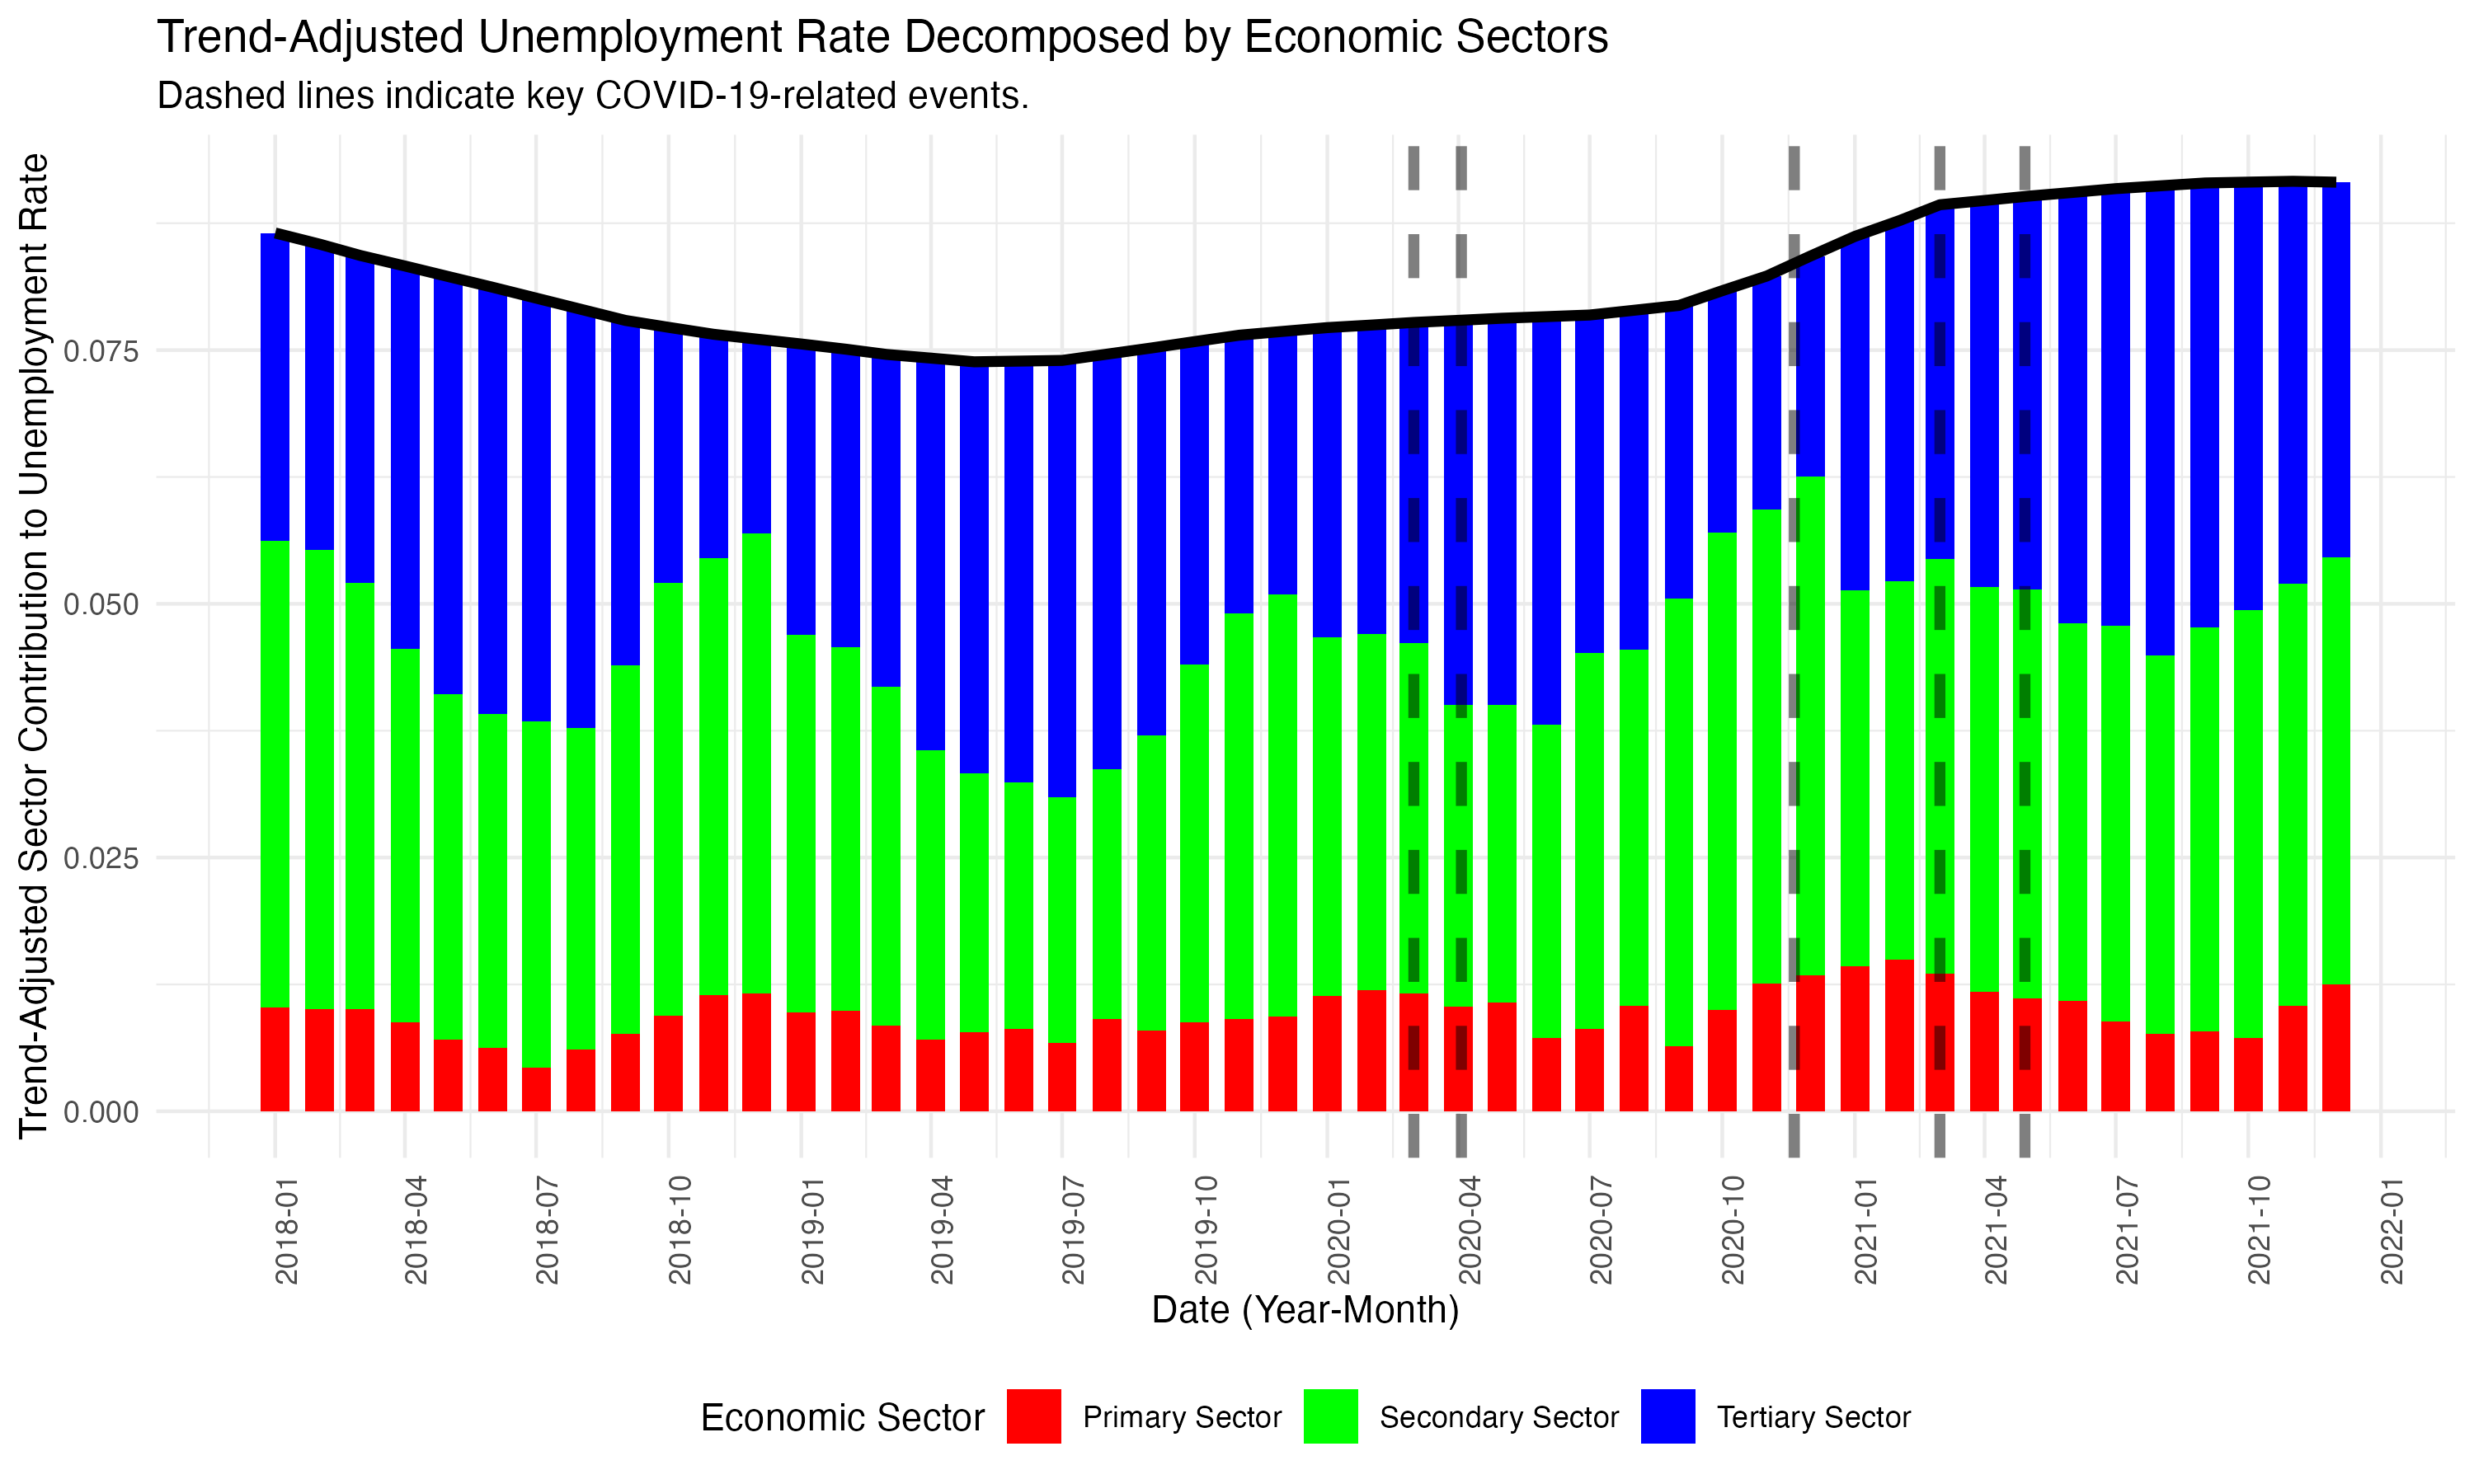
\includegraphics[width=0.8\linewidth]{trend_adjusted_plot.png}
        \caption{Trend Adjusted Unemployment - Sectoral Decomposition}
        \label{fig:trend_adj_threesectors}
    \end{figure}

    \begin{figure} [H]
        \centering
        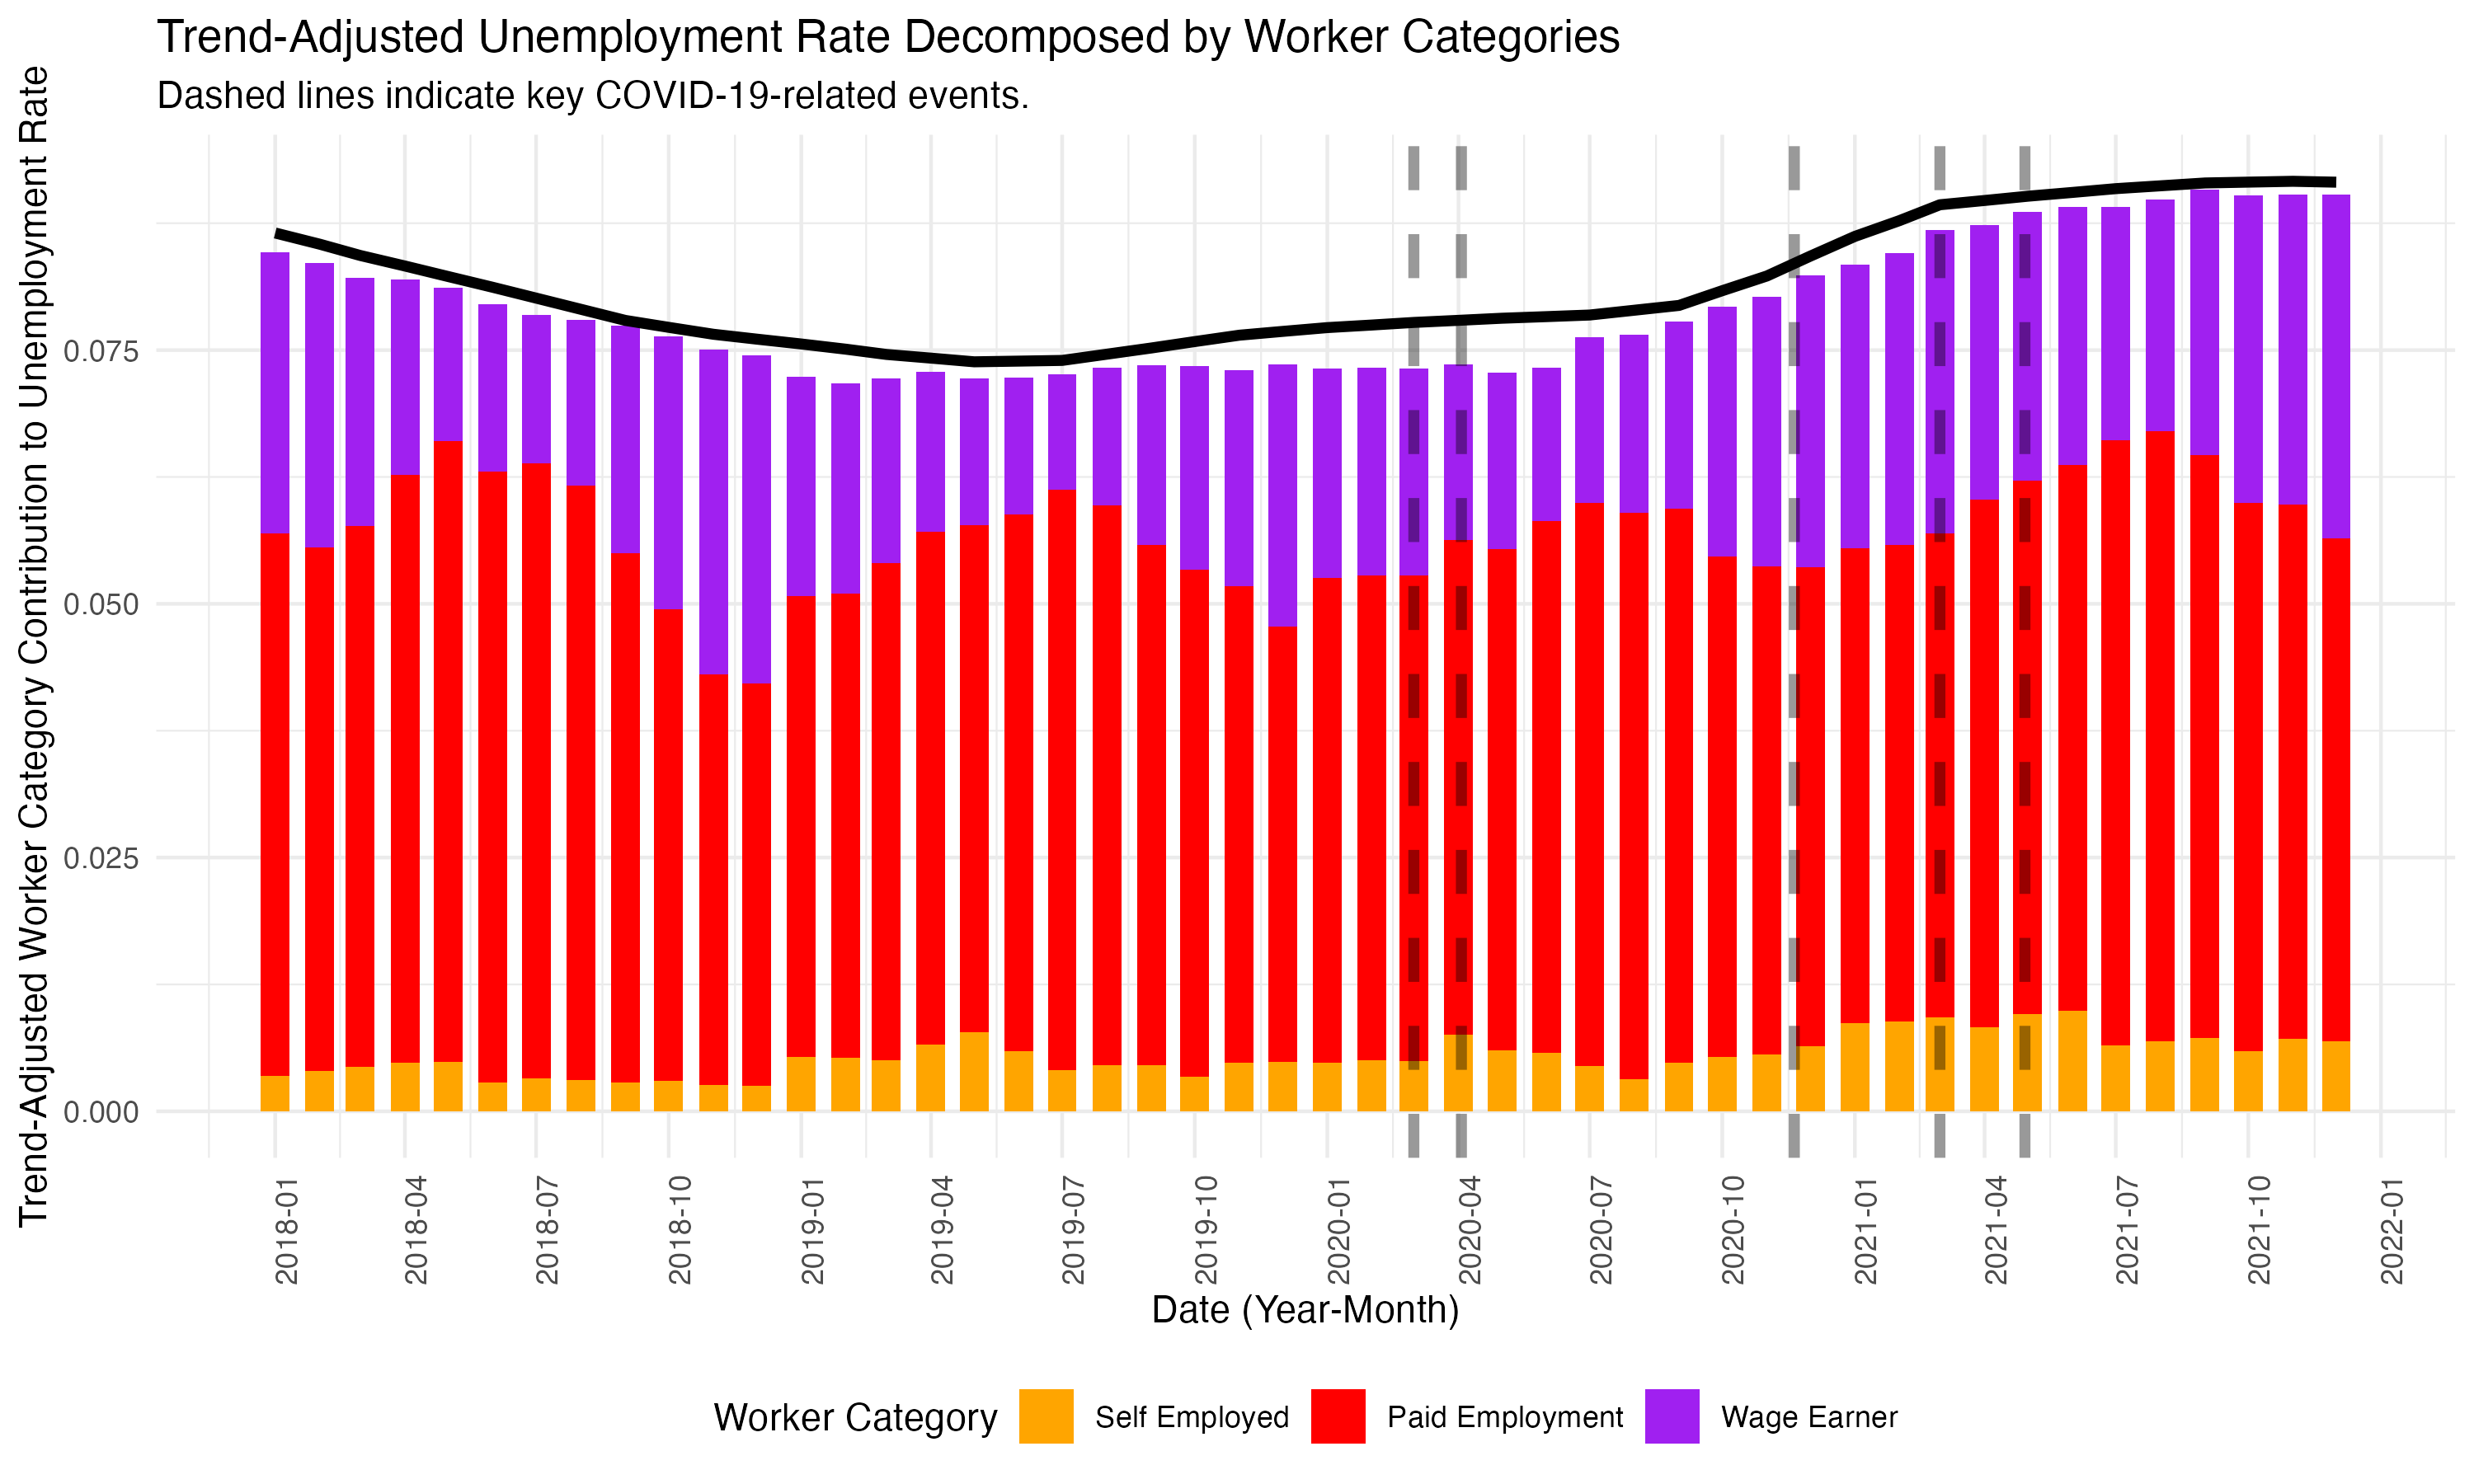
\includegraphics[width=0.8\linewidth]{worker_adjusted_plot.png}
        \caption{Trend Adjusted Unemployment - Employment Types}
        \label{fig:trend_adj_employment}
    \end{figure}

    \begin{figure} [H]
        \centering
        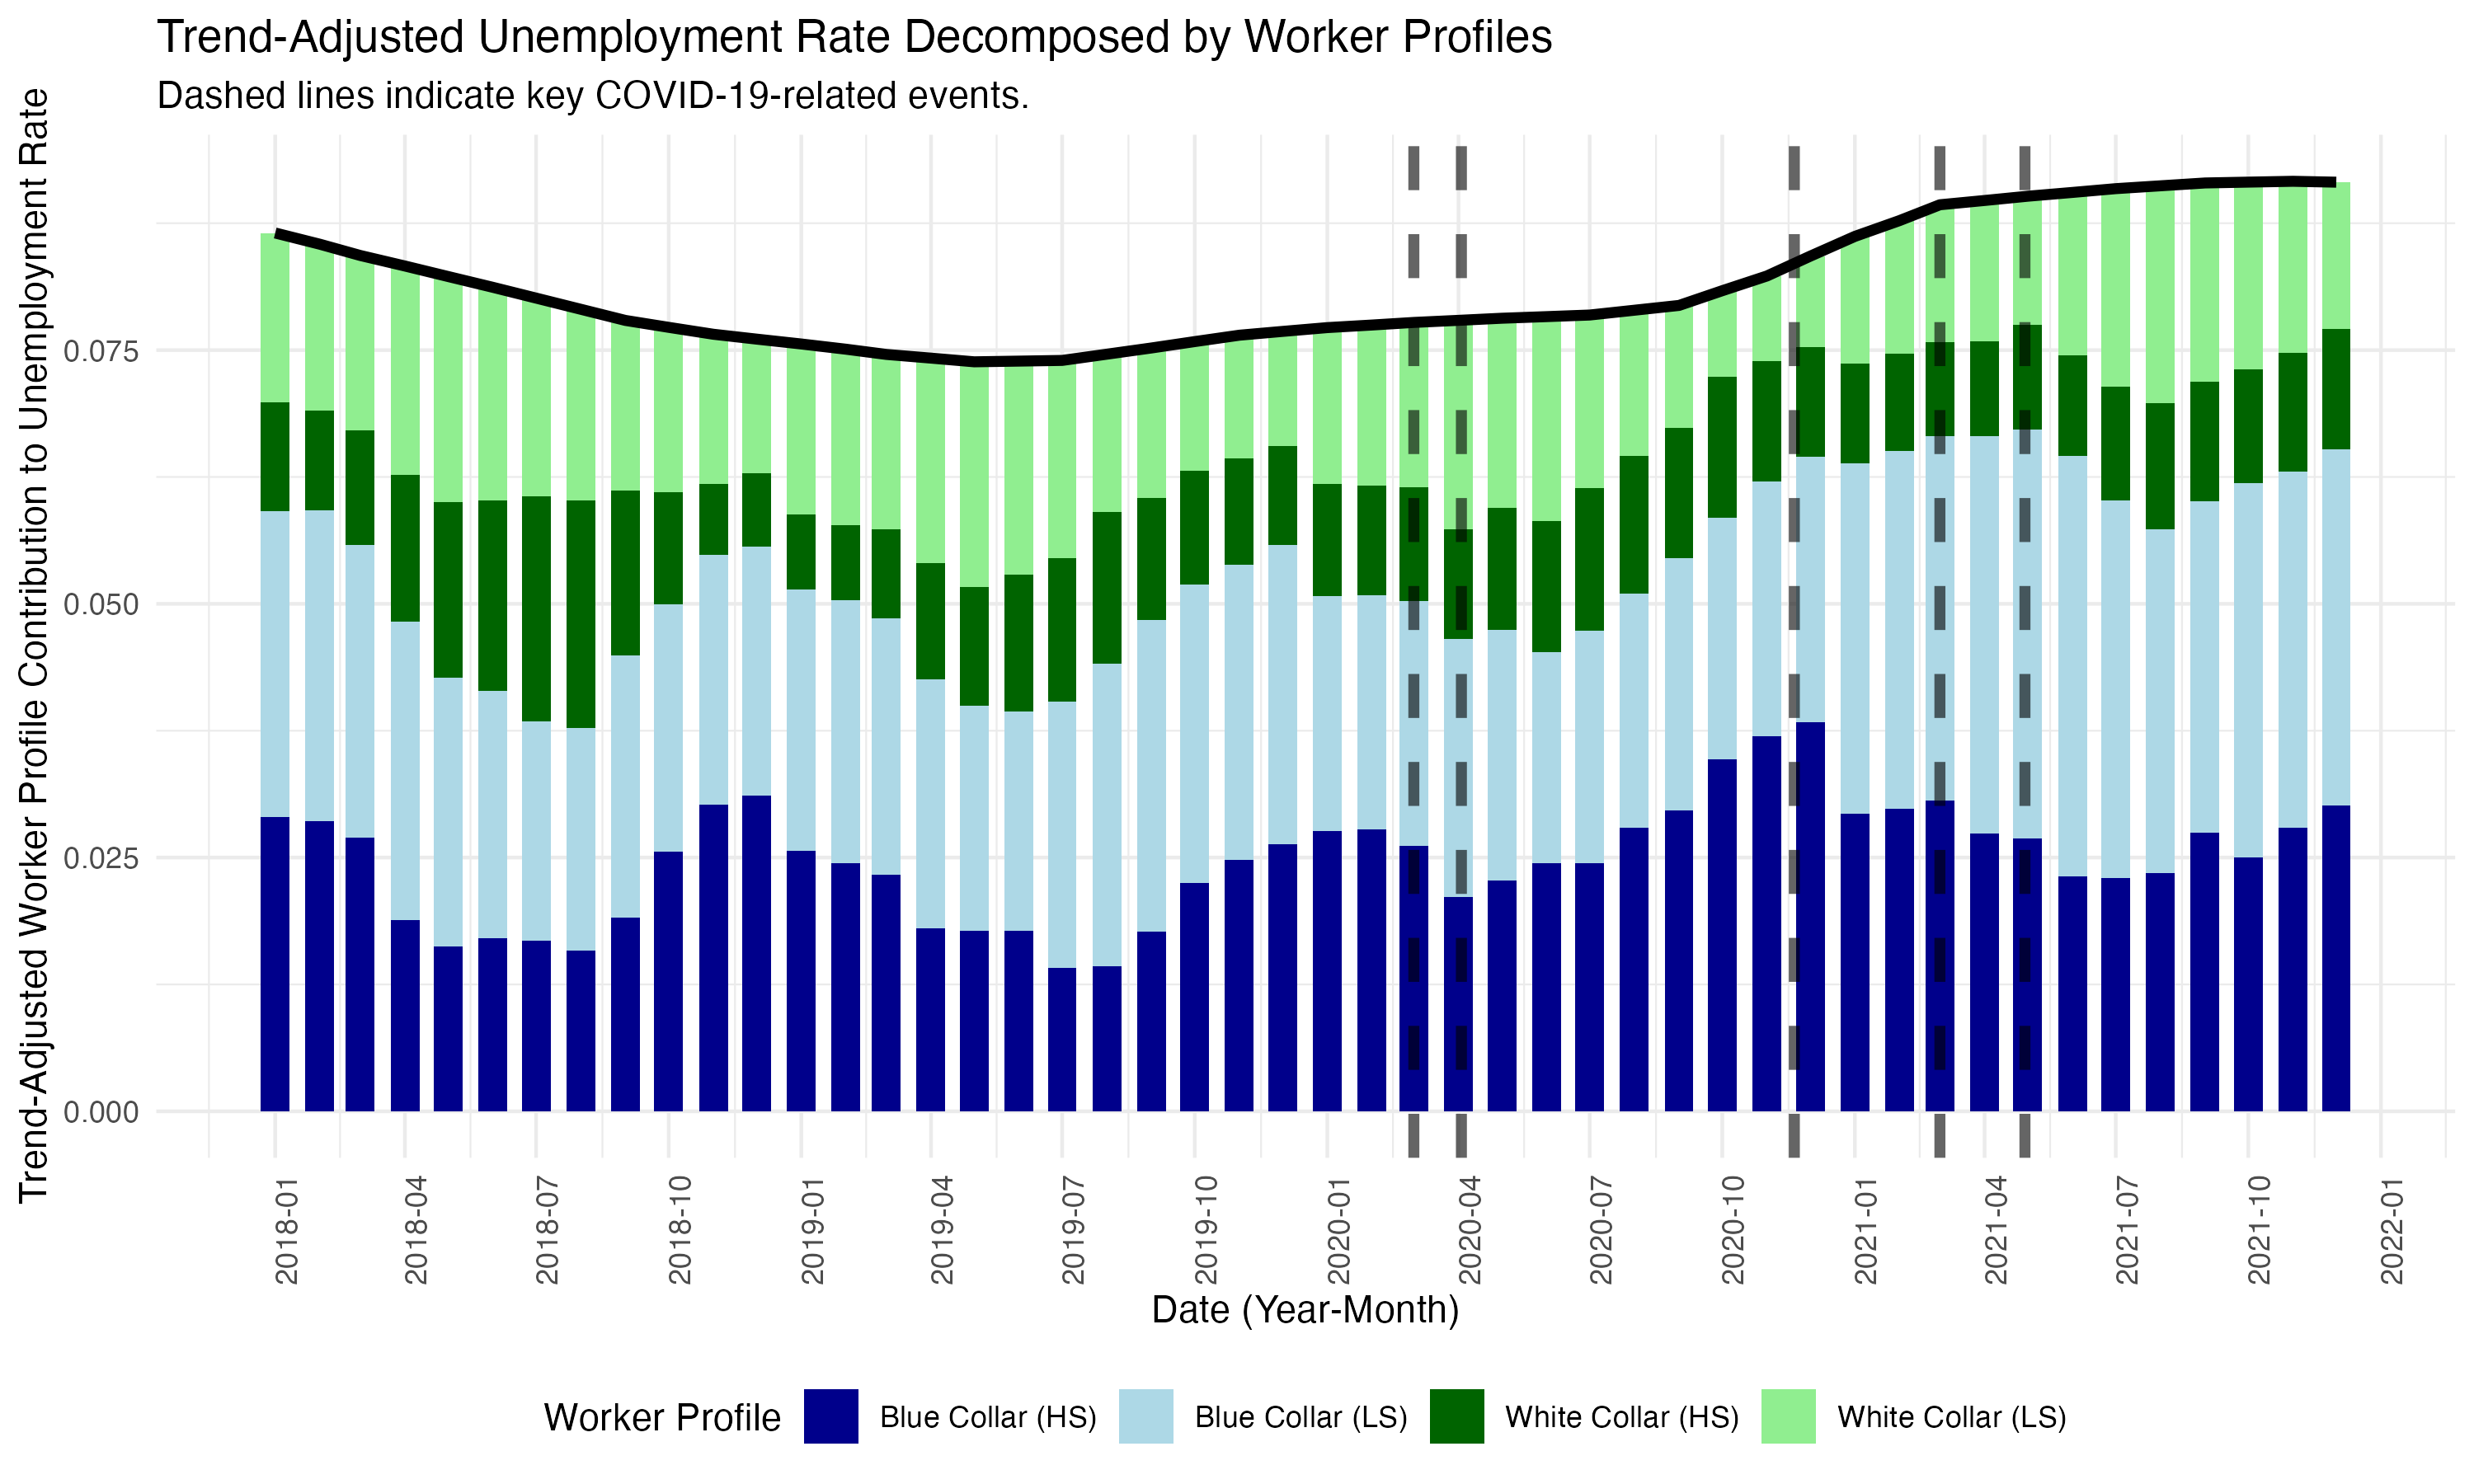
\includegraphics[width=0.8\linewidth]{trend_adj_worker_prof (1).png}
        \caption{Trend Adjusted Unemployment - Worker Profiles}
        \label{fig:trend_adj_worker_prof}
    \end{figure}

    



\subsection{Centered Log-Ratio Transformation} \label{appendix:clr_math}

For a compositional vector 
\[
\mathbf{x} = [x_1, x_2, \dots, x_D]
\]
where \( x_i > 0 \) and 
\[
\sum_{i=1}^{D} x_i = k \quad (\text{e.g., } k = 1 \text{ for proportions or } k = 100 \text{ for percentages}),
\]
the CLR transformation is given by:
\[
\text{CLR}(\mathbf{x}) = \left[ \log \left( \frac{x_1}{g(\mathbf{x})} \right), \log \left( \frac{x_2}{g(\mathbf{x})} \right), \dots, \log \left( \frac{x_D}{g(\mathbf{x})} \right) \right]
\]
where \( g(\mathbf{x}) \) is the geometric mean of the components:
\[
g(\mathbf{x}) = \left( \prod_{i=1}^{D} x_i \right)^{1/D}
\]


\subsection{Clustering Methodology}
\label{appendix:clustering_methodology}

\subsubsection{Hierarchical Clustering}
Hierarchical clustering involves constructing a hierarchy of clusters. The steps followed are:
\begin{enumerate}
    \item Compute the distance matrix for the dataset using Euclidean distance.
    \item Apply a linkage method (e.g., single, complete, average) to iteratively merge clusters.
    \item Visualize the clustering structure through a dendrogram (Figure~\ref{fig:hierarchical-dendrogram}).
    \item Determine the appropriate number of clusters by cutting the dendrogram at a desired height.
\end{enumerate}

\begin{figure} [H]
    \centering
    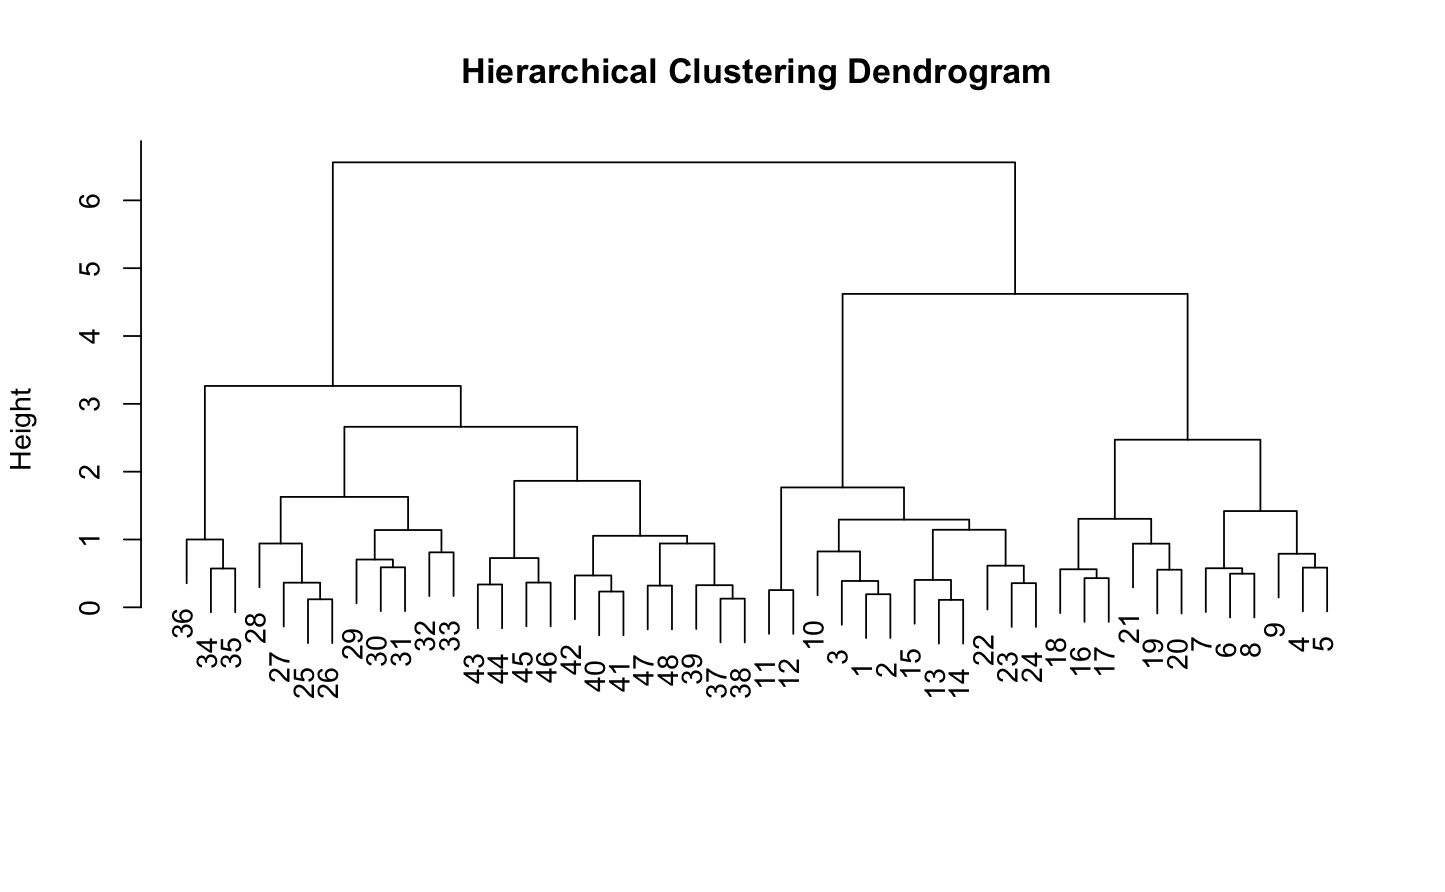
\includegraphics[width=0.8\linewidth]{clr_hier_dendo.png}
    \caption{Dendogram for Hierarchical Clustering Method}
    \label{fig:hierarchical-dendrogram}
\end{figure}

\subsubsection{K-Means Clustering}
K-means clustering partitions data into a predefined number of \(k\) clusters. The steps are:
\begin{enumerate}
    \item Initialize \(k\) cluster centroids randomly.
    \item Assign each data point to the nearest cluster centroid based on Euclidean distance.
    \item Update the cluster centroids by computing the mean of all points assigned to each cluster.
    \item Repeat steps 2 and 3 until convergence or until the centroids stabilize.
    \item Use the elbow method (Figure~\ref{fig:elbow_method}) to identify the optimal number of clusters.
\end{enumerate}

\begin{figure} [H]
    \centering
    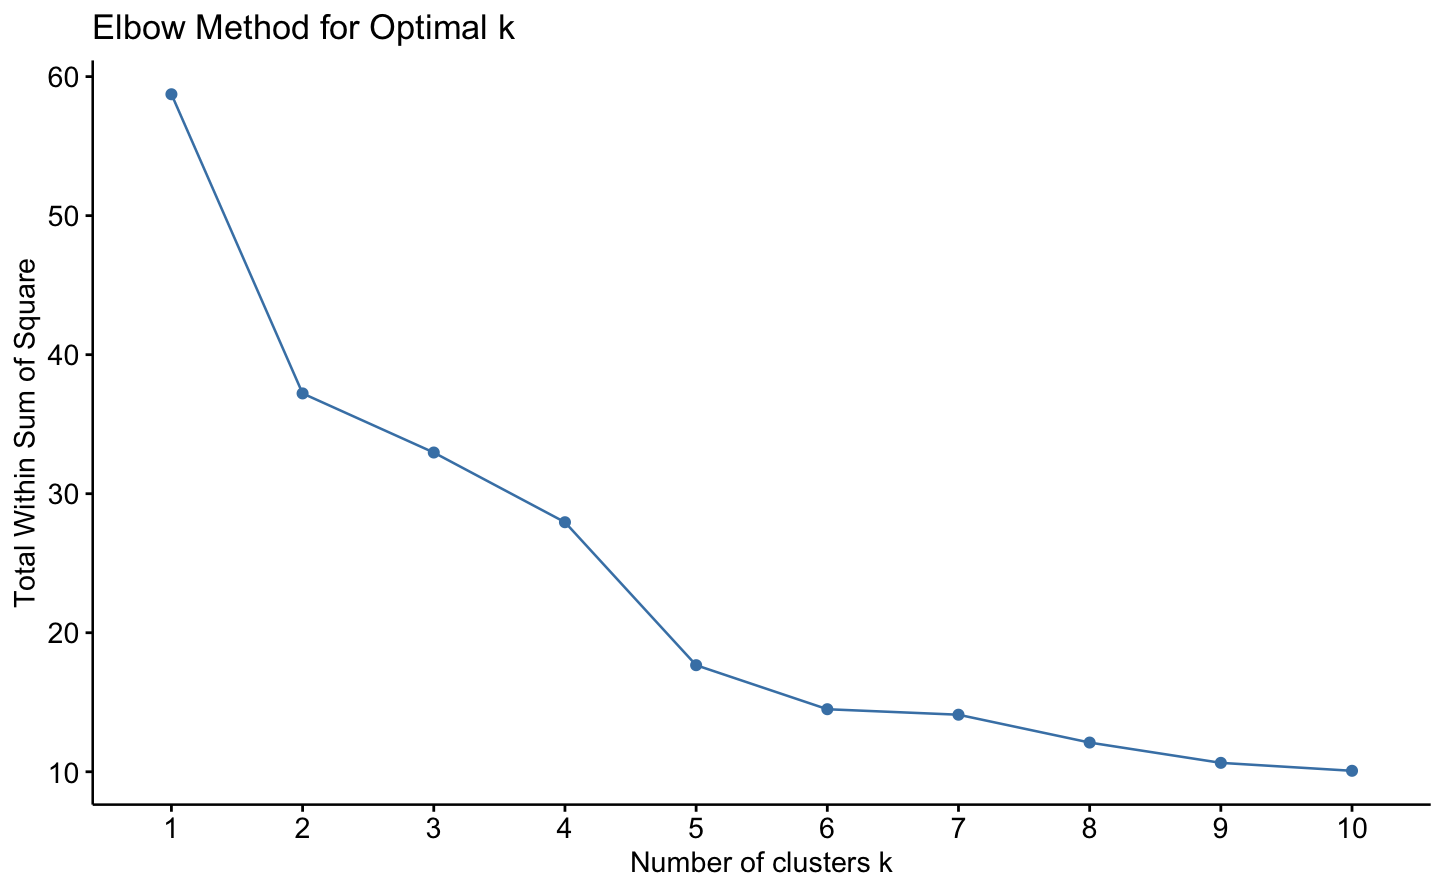
\includegraphics[width=0.8\linewidth]{elbow method.png}
    \caption{Elbow Method for k-mean Clustering Method}
    \label{fig:elbow_method}
\end{figure}


\subsubsection{Comparison of Clustering Methods}

\begin{table}[H]
\centering
\begin{tabular}{|l|p{6cm}|p{6cm}|}
\hline
\textbf{Feature}       & \textbf{Hierarchical Clustering}                          & \textbf{K-Means Clustering}                     \\ \hline
\textbf{Approach}      & Constructs a hierarchy of nested clusters, visualized through a dendrogram. & Partitions data into $k$ clusters iteratively based on minimizing within-cluster variance. \\ \hline
\textbf{Input Requirement} & Distance matrix or raw data.                            & Raw data and predefined number of clusters ($k$). \\ \hline
\textbf{Output}        & Dendrogram and clusters determined at a chosen hierarchical level. & Final cluster assignments and cluster centroids. \\ \hline
\textbf{Sensitivity}   & Stable across seeds; results depend on the chosen linkage method (e.g., single, complete, average). & Sensitive to initial seed choice; faster but less stable, with possible convergence to local optima. \\ \hline
\textbf{Use Case}      & Suitable for smaller datasets or when the number of clusters is unknown. & Best for large datasets when the desired number of clusters is specified. \\ \hline
\end{tabular}
\caption{Comparison of Hierarchical and K-Means Clustering Methods.}
\label{tab:clustering-comparison}
\end{table}


\end{document}